\documentclass[embargoed]{grattan}

\usepackage{relsize}
\usepackage[toc,acronym]{glossaries}
\newcommand*{\abbrev}[1]{{\relsize{-0.5}\uppercase{#1}}}
\defglsentryfmt[acronym]{\abbrev{\glsentrytext{\glslabel}}}
%\renewcommand*{\acronymfont}[1]{\abbrev{#1}}
\newacronym{ABS}{ABS}{Australian Bureau of Statistics}
\newacronym{AGA}{AGA}{Australian Government Actuary}
\newacronym{ATO}{ATO}{Australian Taxation Office}
\newacronym{AWE}{AWE}{Average weekly earnings}
\newacronym{CPI}{CPI}{Consumer price index}
\newacronym{EFTSL}{EFTSL}{Equivalent full-time student load}
\newacronym{FEEHELP}{FEE-HELP}{HELP for full-fee students}
\newacronym{HECS}{HECS}{Higher Education Contribution Scheme}
\newacronym{HECSHELP}{HECS-HELP}{HELP for Commonwealth-supported students}
\newacronym{HELP}{HELP}{Higher Education Loan Program}
\newacronym{HESA}{HESA}{Higher Education Support Act 2003}
\newacronym{OSHELP}{OS-HELP}{HELP to finance overseas study}
\newacronym{PAYG}{PAYG}{Pay As You Go taxation}
\newacronym{SAHELP}{SA-HELP}{HELP for the student amenities fee}
\newacronym{VETFEEHELP}{VET FEE-HELP}{HELP for vocational diplomas and advanced diplomas}


% \newglossaryentry{ACER}{
% 	name = {ACER},
% 	description = {Australian Council for Educational Research}}
% \newglossaryentry{ACPET}{
% 	name = {ACPET},
% 	description = {Australian Council for Private Education and Training}}
% \newglossaryentry{Applied research}{
% 	name = {Applied research},
% 	description = {Research undertaken primarily to acquire new knowledge with a specific application in view.}}
% \newglossaryentry{AQF}{
% 	name = {AQF},
% 	description = {Australian Qualifications Framework}}
% \newglossaryentry{ANZSCO}{
% 	name = {ANZSCO},
% 	description = {Australian and New Zealand Standard Classification of Occupations}}
% \newglossaryentry{ARC}{
% 	name = {ARC},
% 	description = {Australian Research Council}}
% \newglossaryentry{ARWU}{
% 	name = {ARWU},
% 	description = {Academic Ranking of World Universities}}
% \newglossaryentry{ASCED}{
% 	name = {ASCED},
% 	description = {Australian Standard Classification of Education}}
% \newglossaryentry{ATAR}{
% 	name = {ATAR},
% 	description = {Australian Tertiary Admission Rank}}
% \newglossaryentry{ATN}{
% 	name = {ATN},
% 	description = {Australian Technology Network}}
% \newglossaryentry{ATO}{
% 	name = {ATO},
% 	description = {Australian Taxation Office}}
% \newglossaryentry{CGS}{
% 	name = {CGS},
% 	description = {Commonwealth Grant Scheme}}
\newglossaryentry{Commonwealth supported}{
	name = {Commonwealth supported},
	description = {A higher education enrolment funded by the Commonwealth Grant Scheme or required to pay student contribution}}
\newglossaryentry{Doubtful debt}{
	name = {Doubtful debt},
	text = {doubtful debt},
	description = {HELP debt not expected to be repaid}}
% \newglossaryentry{EFTSL}{
% 	name = {EFTSL},
% 	description = {Equivalent full-time student load}}
% \newglossaryentry{ERA}{
% 	name = {ERA},
% 	description = {Excellence in Research for Australia}}
% \newglossaryentry{Experimental development research}{
% 	name = {Experimental development research},
% 	description = {Research using existing knowledge gained from research or practical experience, which is directed to producing new materials, products, devices, policies, behaviours or outlooks.}}
% \newglossaryentry{FEE-HELP}{
% 	name = {FEE-HELP},
% 	description = {HELP for full-fee students}}
\newglossaryentry{Fiscal balance}{
	name = {Fiscal balance},
	text = {fiscal balance},
	description = {An accrual measure of the government's revenue less expenditure}
}
% \newglossaryentry{FTE}{
% 	name = {FTE},
% 	description = {Full-time equivalent}}
% \newglossaryentry{GCA}{
% 	name = {GCA},
% 	description = {Graduate Careers Australia}}
% \newglossaryentry{Group of Eight}{
% 	name = {Group of Eight},
% 	description = {Coalition of Australia's `sandstone' universities}}
% \newglossaryentry{HECS}{
% 	name = {HECS},
% 	description = {Higher Education Contribution Scheme}}
% \newglossaryentry{HECS-HELP}{
% 	name = {HECS-HELP},
% 	description = {HELP for Commonwealth-supported students}}
% \newglossaryentry{HELP}{
% 	name = {HELP},
% 	description = {Higher Education Loan Program}}
% \newglossaryentry{HEP}{
% 	name = {HEP},
% 	description = {Higher Education Provider}}
% \newglossaryentry{HILDA}{
% 	name = {HILDA},
% 	description = {Household, Income and Labour Dynamics in Australia Survey}}
% \newglossaryentry{ICT}{
% 	name = {ICT},
% 	description = {Information and communications technology}}
% \newglossaryentry{IRU}{
% 	name = {IRU},
% 	description = {Innovative Research Universities}}
% \newglossaryentry{IT}{
% 	name = {IT},
% 	description = {Information technology}}
% \newglossaryentry{Load}{
% 	name = {Load},
% 	description = {Subjects taken, expressed in full-time student units.}}
\newglossaryentry{Interest subsidy}{
	name = {Interest subsidy},
	text = {interest subsidy},
	description = {Subsidies provided by the government to HELP debtors for providing loans at a discounted interest rate}}
\newglossaryentry{Loan fees}{
	name = {Loan fees},
	text = {loan fees},
	description = {Charges added to new outstanding debt for borrowing through HELP to be repaid under the same repayment setting as the principal}}
% \newglossaryentry{NUHEP}{
% 	name = {NUHEP},
% 	description = {Non-university higher education provider}}
% \newglossaryentry{OS-HELP}{
% 	name = {OS-HELP},
% 	description = {HELP to finance overseas study}}
% \newglossaryentry{OUA}{
% 	name = {OUA},
% 	description = {Open Universities Australia}}
% \newglossaryentry{Pathway college}{
% 	name = {Pathway college},
% 	description = {Institution specialising in diploma level courses aimed at facilitating entry to university courses.}}
% \newglossaryentry{Place}{
% 	name = {Place},
% 	description = {A student place is equivalent to the study load of a full-time student}}
% \newglossaryentry{Pure basic research}{
% 	name = {Pure basic research},
% 	description = {Research to acquire new knowledge without looking for long term benefits other than advancing knowledge.}}
% \newglossaryentry{RUN}{
% 	name = {RUN},
% 	description = {Regional Universities Network}}
% \newglossaryentry{SA-HELP}{
% 	name = {SA-HELP},
% 	description = {HELP for the student amenities fee}}
% \newglossaryentry{SES}{
% 	name = {SES},
% 	description = {Socio-economic status}}
% \newglossaryentry{Strategic basic research}{
% 	name = {Strategic basic research},
% 	description = {Research in specified areas in the expectation of practical discoveries.}}
% \newglossaryentry{STEM}{
% 	name = {STEM},
% 	description = {Science, technology, engineering and mathematics}}
\newglossaryentry{Student contribution}{
	name = {Student contribution},
	text = {student contribution},
	description = {The amount paid by a student in a Commonwealth-supported place}}
% \newglossaryentry{TAFE}{
% 	name = {TAFE},
% 	description = {Technical and further education}}
% \newglossaryentry{TEQSA}{
% 	name = {TEQSA},
% 	description = {Tertiary Education Quality and Standards Agency}}
\newglossaryentry{Threshold}{
	name = {Threshold},
	text = {threshold},
	description = {Income level that triggers HELP repayment or a new rate of repayment}}

\makeglossaries

\usepackage{soul}
\usepackage{bbding}
%\newcommand{\warn}[1]{\GenericWarning{LaTeX Warning: #1}{LaTeX Warning: #1}{\textcolor{red}{\XSolidBold} #1 \textcolor{red}{\XSolidBold}}}

\newcommand{\warn}[1]{\GenericWarning{LaTeX Warning: #1}{LaTeX Warning: #1}\textcolor{red}{\XSolidBold} \hl{#1} \textcolor{red}{\XSolidBold}}



% Person-specific margin comments
\usepackage{todonotes}
\setlength{\marginparwidth}{1.8cm}

\newcommand{\ittima}[1]{\todo[color=Color2,size=\scriptsize]{\textbf{Ittima:} #1}\ }
\newcommand{\andrew}[1]{\todo[color=Color3,size=\scriptsize]{\textbf{Andrew:} #1}\ }
\newcommand{\john}[1]{\todo[color=Color1,size=\scriptsize]{\textbf{John:} #1}\ }

% Inline comments (for environments)
\newcommand{\ittimai}[1]{\todo[color=Color2,size=\scriptsize,inline]{\textbf{Ittima:} #1}}
\newcommand{\andrewi}[1]{\todo[color=Color3,size=\scriptsize,inline]{\textbf{Andrew:} #1}}
\newcommand{\johni}[1]{\todo[color=Color1,size=\scriptsize,inline]{\textbf{John:} #1}}
\addbibresource{bib/HE-Bib.bib}

\title{Shared interest: A universal loan fee for \gls{HELP}}
\author{Andrew Norton and Ittima Cherastidtham}

\EmbargoDate{December 4 2016}

\GrattanReportNumber{2016-17}


\acknowledgements{%
This report was written by 
Andrew Norton, Grattan Institute Higher Education Program Director, and Ittima Cherastidtham, Grattan Institute Senior Associate. 

We would like to thank Tim Higgins and an anonymous reviewer for detailed comments on the report, and members of Grattan Institute's Higher Education Program Reference Group for their helpful comments.

The opinions in this report are those of the authors and do not necessarily represent the views of Grattan Institute's founding members, affiliates, individual board members reference group members or reviewers.
Any remaining errors or omissions are the responsibility of the authors.

Grattan Institute is an independent think-tank focused on Australian public policy.
Our work is independent, practical and rigorous.
We aim to improve policy outcomes by engaging with both decision-makers and the community.

Andrew Norton’s higher education reports are notified via Twitter, @andrewjnorton, and through the Grattan Institute’s mailing list. To join it, please go to: 
\textcolor{blue}{\url{http://www.grattan.edu.au/}}.


{\footnotesize
This report may be cited as:\\
Norton, A. and Cherastidtham, I., 2016, \emph{Shared interest: A universal loan fee for \gls{HELP}}, Grattan Institute

ISBN: 978-1-925015-97-3

All material published or otherwise created by Grattan Institute is licensed under a Creative Commons Attribution-NonCommercial-ShareAlike 3.0 Unported License\par
}
\AtEndDocument{\footnotesize\RaggedRight
This paper uses unit record data from the Household, Income and Labour Dynamics in Australia (HILDA) Survey.
The HILDA project was initiated and is funded by the Australian Government Department of Social Services (DSS) and is managed by the Melbourne Institute of Applied Economic and Social Research.
The findings and views reported in this paper, however, are those of the authors and should not be attributed to DSS or the Melbourne Institute.\par
}
}



\begin{document}

\setlength{\overviewExtra}{-2pt}
\begin{overview}
Introduced in 1989, \gls{HELP} has greatly expanded access to tertiary education.
Students can finance their education by taking out \gls{HELP} loans.
By requiring students to contribute financially, the government can spread its limited resources across more students.

But financing these loans is costly for taxpayers.
Every year the government pays the difference between the \gls{CPI} interest it charges students and the cost of its own borrowing to finance government debt.

As of mid-2016, total \gls{HELP} debt is about \$52~billion.
The interest subsidy on this debt is about \$600~million.
This cost will escalate as total \gls{HELP} debt grows and interest rates increase.
The government currently pays a low interest rate on its debt, but this could increase by 60 per cent if rates return to their average over the last ten years.

The government could recover most of its interest costs by charging loan fees on all new \gls{HELP} lending.
Some students already pay loan fees, which are added to their total debt when they borrow.
A universal 15 per cent loan fee paid by all \gls{HELP} borrowers would have saved \$700~million in 2016.

The universal loan fee would replace existing loan fees.
Full-fee vocational education and undergraduate students pay loan fees of 20 and 25 per cent respectively while postgraduate and government-supported students do not.
These loan fee differences among students are unfair and lack a policy rationale.

Loan fees preserve \gls{HELP}'s policy goals.
Cash-poor students can continue to borrow with no upfront charges.
Low-income graduates would continue to repay nothing until their income reaches the \gls{HELP} threshold, which is currently \$54,869.
For repaying \gls{HELP} debtors, loan fees would extend their repayment period but leave annual repayments unchanged.

Interest subsidies are not well targeted.
Although low-income \gls{HELP} debtors receive the highest subsidies, affluent graduates receive about 10 per cent of their original borrowing in subsidies.
Their earnings average more than \$120,000 a year.
The case for subsidising them is weak.

A universal 15 per cent loan fee would cover the government's expected average interest cost for repaying graduates.
High income graduates who repay quickly would more than cover their interest costs, and would cross-subsidise the cost of low-income graduates who repay slowly.

Loan fees are progressive compared to previously proposed real interest rates on \gls{HELP} loans.
Under real interest rates, debtors taking breaks from work or earning low incomes pay more interest than high-income earners with the same original debt.
Under loan fees, interest charges vary with the amount borrowed but not with how long it takes to repay.

With both the current and the previous government looking to reduce higher education spending, we need savings that are consistent with educational and social goals.
Loan fees leave per student university funding unchanged, reduce pressure to cap student numbers, avoid upfront charges, and preserve protections for low-income graduates.
\end{overview}

\contentspage



\chapter{{Introduction}}\label{chap:1-introduction}

More than four million Australians have borrowed to finance their tertiary education through the Higher Education Loan Program (HELP).
Introduced in 1989, it helps cash-poor students finance their education and repay later when they are better off.

\gls{HELP}'s main feature is its income-contingency.
Debtors who earn below the repayment threshold are not required to repay.
Those who earn at least the repayment threshold -- \$54,869 in 2016-17 -- repay 4 per cent of their income.
The proportion of income repaid increases as income rises.

While income-contingent repayment benefits students, it creates costs for the government.
\gls{HELP} debt is indexed to \gls{CPI}.
Since the government's borrowing cost tends to be higher than inflation, the government subsidises the interest costs.
The slower debtors are to repay, the higher the subsidies.

As of mid-2016, more than \$52~billion of \gls{HELP} debt was outstanding.
The interest cost is more than \$600~million for 2015-16.

As \Chapref{chap:2-helps-interest-costs} explains, subsidies are likely to quickly escalate.
The gap between the government's borrowing cost and \gls{CPI} -- known as the real interest rate -- is low at present compared to its historical average.
The low rate masks a potential 60 per cent cost increase if the rate returns to its average over the last ten years.

High levels of debt also increase interest costs.
While lending for vocational education is reducing, for higher education it continues to increase.
Repayments of \gls{HELP} debt have grown slowly in recent years.

No public government document describes who receives interest subsidies.
\Chapref{chap:3-who-receives-interest-subsidies} uses the 2011 Census to estimate the lifetime interest cost of working bachelor degree graduates.
The average interest subsidy is 17 per cent of initial borrowing for women and 16 per cent for men.

While subsidies flow more to low-income graduates than to those on high incomes, they are not well targeted.
Debtors who earn high incomes receive about 10 per cent of their initial borrowing in subsidies.
Most earn more than \$120,000 a year by their late twenties.
The case for subsidising them is weak.

\gls{HELP} manages student and debtor risks and smooths their living standards.
\Chapref{chap:4-does-help-need-interest-subsidies} argues that interest subsidies are not needed to achieve these purposes as long as repayments are income-contingent.

From the government's perspective, the subsidy generates more lending than necessary.
Many postgraduates are able to pay upfront but tend to borrow.

While \gls{HELP} is not meant to recover all its costs, it should put fewer demands on the Budget by reducing interest subsidies.
Yet not all methods of recovering interest subsidies are equal.
In 2014 the Abbott government proposed charging real interest on \gls{HELP}.
Rather than indexing \gls{HELP} to \gls{CPI}, it would have been indexed it to the government's cost of borrowing.
The reform would have increased repayments and reduced cost.

But as \Chapref{chap:5-charging-real-interest} argues, indexing \gls{HELP} debt to real interest disproportionately affects low-income graduates compared to high-income graduates who repay.
Women who leave the workforce to have children would repay more than those who don't.
A hybrid model -- a model that indexes \gls{HELP} to a mix of inflation-only and real interest -- can address some of these problems.
But it cannot eliminate them.

\Chapref{chap:6-loan-fee} proposes charging loan fees rather than indexing \gls{HELP} to real interest.
Even though \gls{HELP} already has loan fees for some students, the inconsistent rates across programs are difficult to justify.
We recommend charging a 15 per cent loan fee across all programs, regardless of qualification or higher education provider.
In 2016 the government is expected to lend \$8~billion.
A 15 per cent loan fee would raise nearly \$1.2~billion to offset interest costs over the life of student loans.
This would lead to \$700~million in savings, after reducing existing loan fees.

\Chapref{chap:6-loan-fee} also investigates how loan fees are consistent with \gls{HELP}'s social goals.
Because \gls{HELP}'s repayments are income contingent, debtors with low incomes would continue to be protected from repaying.
The likely effects on demand of charging loan fees, and therefore \gls{HELP}'s goal of ensuring access to education, are small.

\chapter[HELP's interest costs]{\gls{HELP}'s interest costs}\label{chap:2-helps-interest-costs}

Interest subsidies are one of \gls{HELP}'s major costs.
As outstanding \gls{HELP} debt grows so do interest subsidies.
This chapter describes existing \gls{HELP} interest subsidies and the long-term trends affecting interest costs.

\section[CPI versus the government's cost of borrowing]{\gls{CPI} versus the government's cost of borrowing}\label{sec:cpi-versus-the-governments-cost-of-borrowing}

Since its introduction in 1989, \gls{HECS} and subsequently \gls{HELP} loans have been indexed to the consumer price index \gls{CPI}.
Indexation ensures that \gls{HELP} balances keep their real value in the face of inflation.
But the government's cost of financing these loans is generally higher than inflation.%
\footnote{HELP lending, tuition funding, and most other higher education programs are special appropriations from consolidated government revenue.
The government therefore does not borrow specifically for \gls{HELP}, but \gls{HELP} requires it to borrow more than it otherwise would if students were required to pay their student charges upfront.}

The difference between the government's cost of borrowing and inflation is an interest subsidy.
So if the government pays 5 per cent interest on its debt and \gls{CPI} is 2 per cent, the subsidy is 3 per cent.
The larger the difference between the two rates the greater the subsidy.
In this report the difference between the two rates is referred to as the real interest rate.

There are different ways of costing interest subsidies.
The government's accounts use the expected cost of real interest over the life of outstanding loans.
The \gls{AGA} uses a simulation model based on income statistics to estimate repayment streams over graduates' lifetimes.
In simplified terms, they estimate how much \gls{HELP} debtors would repay using \gls{CPI} and a real interest rate.
The difference between the two is approximately the expected interest subsidy.%
\footnote{In more technical terms, the \gls{AGA}'s calculation of interest subsidies uses two present values of expected future \gls{HELP} repayments of outstanding loans.
The first present value represents expected repayments discounted by forecast \gls{CPI}.
The second present value is calculated by discounting expected repayments by the government securities' yield curve.
The difference between these two present values represents the expected interest subsidy: ACIL Allen Consulting (2013), appendix A.}

All else being equal, debtors who repay slowly receive greater interest subsidies than those who repay quickly.
Since interest subsidies are based on future repayments, debtors who are not expected to make any repayments incur no interest subsidies.
Their loans are counted as doubtful debt and eventually written off.

\gls{HELP}'s lending costs appear in the government's accounts in two ways.
In the Department of Education and Training's annual budget papers, the expected future interest subsidy costs of loans made that year are included in an overall estimate of annual \gls{HELP} costs.
In the Department's balance sheet, the total value of all outstanding \gls{HELP} debt is written down to arrive at a `fair value'.
As of mid-2016, outstanding \gls{HELP} lending of about \$52 billion was written down by about \$1.2 billion to reflect interest subsidies over the life of these loans.%
\footcite[][176]{Education2016Annualreport}

Another way of valuing the interest subsidy is to calculate the annual cost of holding the \gls{HELP} debt.
Effectively, this is the interest the government would save if all outstanding \gls{HELP} debt were suddenly repaid.
The government can borrow funds in different ways with different borrowing costs, but this report uses the Australian Government 10-year bond rate to estimate interest subsidy costs.
This is the interest rate the government pays on money it borrows for a 10-year period.
The government used this rate as part of its now-abandoned 2014 proposal to charge real interest on student debt.%
\footcite{Australia2014HigherEducationResearch}

The annual interest subsidy cost on outstanding loans was about \$500 million in 2014-15, as \Vref{fig:fig1-annual-interest-subsidy-is-low-compared-to-when-the-real-interest-rate-was-at-its-10-year-hist-avg} shows.%
\footnote{Grattan analysis of \textcites{ABS2015Educationwork2015}{RBA2016Exchangeratesdaily}{RBA2016F21Capitalmarket}} %CC: need to check this one
%\footnote{Grattan analysis of ABS (2015a); RBA (2016a); RBA (2015)} 
The annual subsidy is estimated to grow by 20 per cent, to over \$600~million in 2015-16, largely due to rising outstanding \gls{HELP} debt.
The cost is expected to grow further in future as debt increases.

\begin{figure}
\caption{The annual interest subsidy is low compared to when the real interest rate was at its ten-year historical average}\label{fig:fig1-annual-interest-subsidy-is-low-compared-to-when-the-real-interest-rate-was-at-its-10-year-hist-avg}

\units{Annual interest subsidy on outstanding loan; \$2015-16~million} 
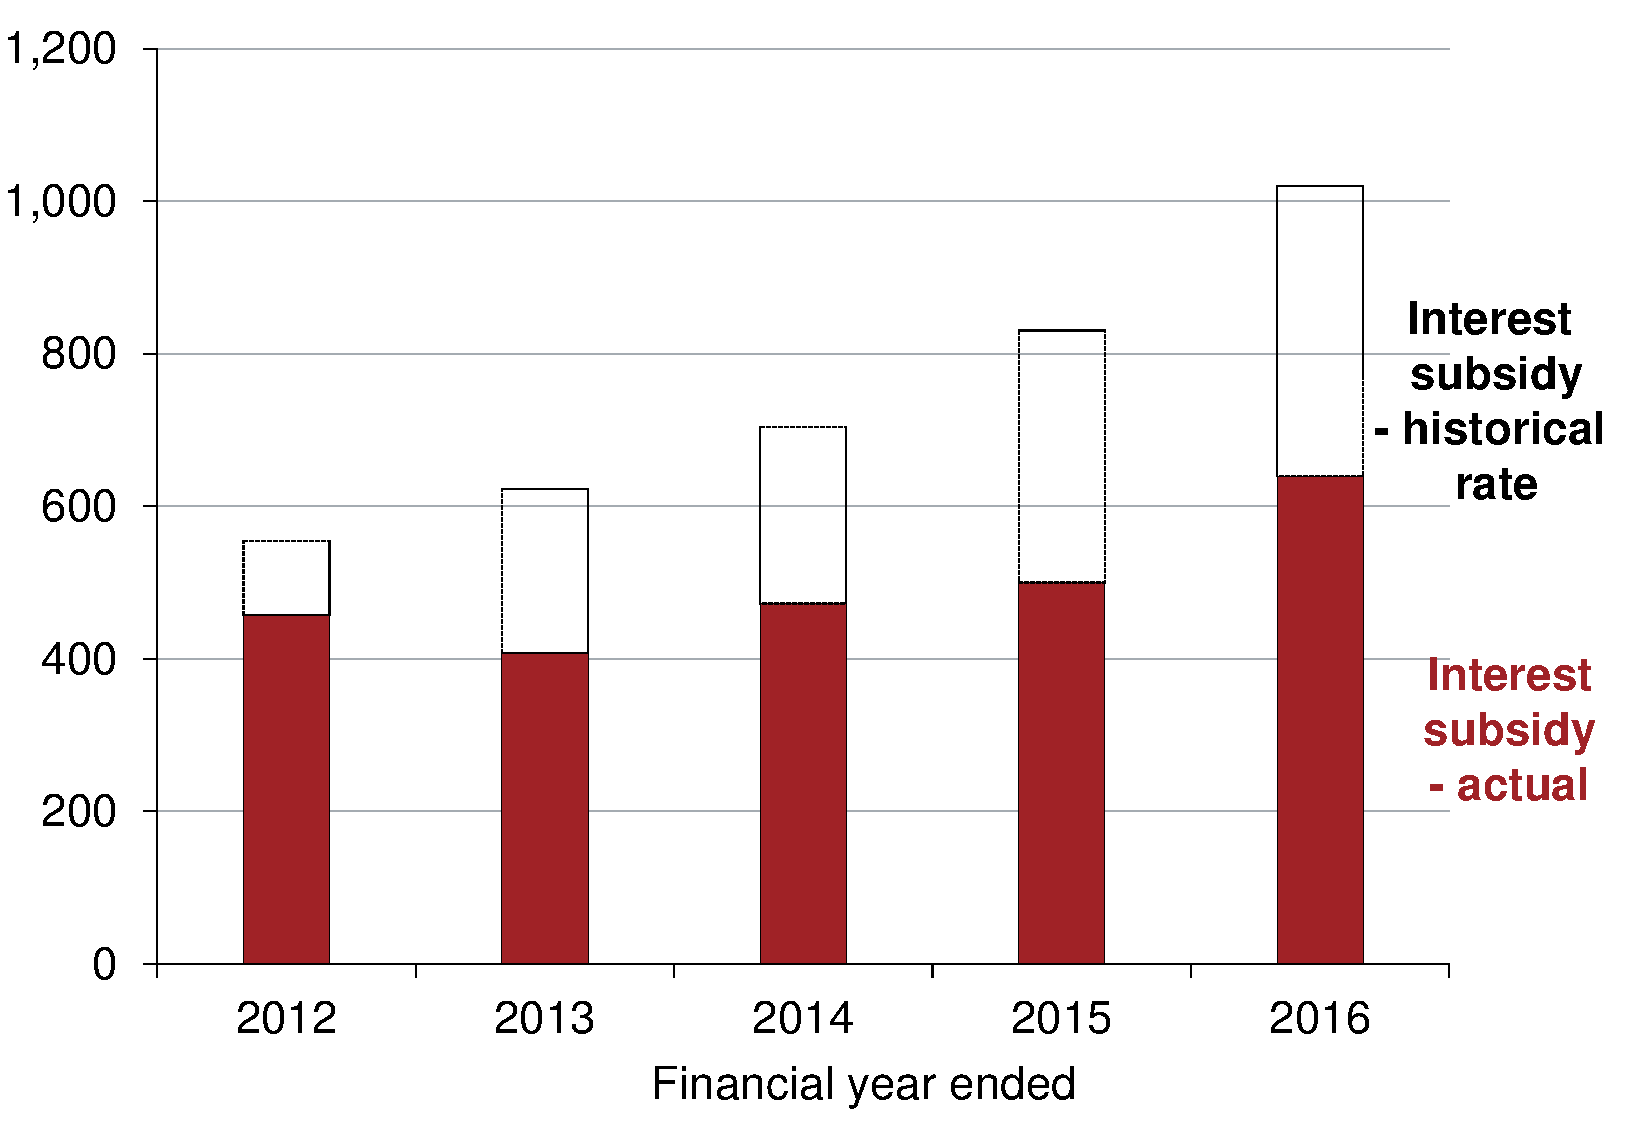
\includegraphics[page=1]{atlas/Chartpack.pdf}

\noteswithsource{%
All groups \gls{CPI} is used.
The calculation of \gls{CPI} is based on the sum of the index numbers for the March quarter in the financial year and of the preceding 3 quarters divided by the sum of the index number for the March quarter for the immediately preceding financial year and the index numbers of the preceding 3 quarters.
It follows the specification in \gls{HESA} 2003.
The calculation of the 10-year bond rate is based on the sum of the yield on the Commonwealth Government 10-year bond for March of the financial year and the yield for the preceding 11 months divided by the sum of the yield for March of the immediately preceding financial year and the yield for the preceding 11 months.
The calculation follows the Higher Education and Research Reform Amendment Bill 2014.
The cost includes all outstanding debt.
The actual annual interest cost represents a lower bound since the government does not immediately index \gls{HELP} lending to \gls{CPI}, the interest cost on new lending would include both \gls{CPI} and real interest.
See footnote \ref{fn:68-High-outstanding-debt-non-fin-impact} on \cpageref{fn:68-High-outstanding-debt-non-fin-impact}.}%
{\textcites{ABS2015Australiandemographicstatistics}{RBA2016Exchangeratesdaily}{EducationvariousyearsHigherEducationStatistics}; Data supplied by the Department of Education and Training.} % CC: check citations
%ABS (2015a); Parliamentary Budget Office (2016); RBA (2016a); Department of Education and Training (various years-a); Data supplied by the Department of Education and Training.}
\end{figure}

\section{Escalating interest cost}\label{escalating-interest-cost}

\begin{figure*}

\begin{minipage}[t][\textheight]{\columnwidth}
\vspace{\grattanfptop}
\caption[The government's cost of borrowing generally exceeds CPI]{The government's cost of borrowing generally exceeds \gls{CPI}}\label{fig:fig2-governments-cost-of-borrowing-exceeds-CPI}
\units{Per cent a year}

\includegraphics[page=2]{atlas/Chartpack.pdf}
\noteswithsource{See \Vref{fig:fig1-annual-interest-subsidy-is-low-compared-to-when-the-real-interest-rate-was-at-its-10-year-hist-avg}.}%
{\textcites{ABS2016ConsumerPriceIndex}{RBA-2015-f2Capitalmarketyields}{RBA2016F21Capitalmarket}}

\end{minipage} \hfill
\begin{minipage}[t][\textheight]{\columnwidth}
\vspace{\grattanfptop}
\caption{The number of government-supported students has doubled since 1989}\label{fig:fig3-number-govt-supported-students-doubled-since-1989}
\units{Number of Commonwealth supported places; full-time equivalent}

\includegraphics[page=3]{atlas/Chartpack.pdf}
\noteswithsource{2015 and 2016 data is an estimate of CGS Commonwealth supported \gls{EFTSL} as at Budget 2016 (May 2016).}%
{Communication from the Department of Education and Training}
\end{minipage}
\end{figure*}

\subsection{Low real interest}\label{low-real-interest}

The Government's interest subsidy costs are moderated at present because the real interest rate is low compared to its historical levels, as \Vref{fig:fig2-governments-cost-of-borrowing-exceeds-CPI} shows.
The 2016 real interest rate is 1.2 per cent.
The average over the last ten years is nearly 2 per cent, and it has occasionally exceeded 4 per cent.%
\footnote{See notes for \Vref{fig:fig1-annual-interest-subsidy-is-low-compared-to-when-the-real-interest-rate-was-at-its-10-year-hist-avg}, \textcite{ABS2016ConsumerPriceIndex}; RBA (2016a); RBA (2015).
The historical average rate is based on the last 10 years.
The 15-year average rate is 2.2 per cent and the 20-year average rate is 2.7 per cent.} The current low rate of interest masks a potential 60 per cent cost increase.

\subsection{Growth in borrowing}\label{subsec:growth-in-borrowing} 

\gls{HELP}, formerly known as \gls{HECS}, has expanded since its introduction 27 years ago.
The most direct descendant of the original \gls{HECS} scheme is \gls{HECSHELP}, which lends to Commonwealth supported students.
Since \gls{HECS} began in 1989, the number of Commonwealth supported students has doubled.
In that year, just over 300,000 places were available for \gls{HECS} students, as \Vref{fig:fig3-number-govt-supported-students-doubled-since-1989} shows.\afterpage{\cleardoublepage} %
This year the government estimates that there are over 600,000 places.
From 2008 limits were progressively removed on how many government-supported bachelor degree places public universities could offer.%
\footnote{Except for medicine} Under this system, now driven by demand, student numbers are likely to keep growing.


As the number of Commonwealth supported students eligible for \gls{HELP} grew so did their tendency to borrow.
Between 2005 and 2015, the proportion of students borrowing increased from 80 to 91 per cent.%
\footnote{Based on \gls{EFTSL} of 2005 onwards students excluding CSP with no \gls{HECSHELP} discount, Department of Education and Training (various years-d), section 5: liability status categories} Borrowing rates are likely to continue increasing, as a discount for paying upfront is abolished from 2017 (\Vref{subsec:little-incentive-to-pay-upfront}).

A change to \gls{HELP} eligibility rules is also likely to reduce upfront payment rates.
Generally, New Zealand citizens are entitled to a Commonwealth supported place and are charged the same amount as Australian students, but cannot borrow under \gls{HELP}.
From 1 January 2016, New Zealand citizens who immigrated when they were less than 18 years old and who have lived in Australia long-term are eligible for \gls{HELP} loans.%
\footnote{Department of Education and Training (2016c)} Some New Zealanders who previously paid upfront are now borrowing.

The growing demands on \gls{HELP} are greater in dollar terms than the increase in borrowers would suggest.
After substantial increases in student charges in 1997 and 2005, an average student borrows much more now than they did originally.%
\footnote{Student contributions are indexed to the Higher Education Grant Index (HEGI); a combination of \gls{CPI} and the wage price index.
From 2018, \gls{CPI} will replace HEGI as a result of the Budget Savings (Omnibus) Bill 2016.} In 1989, the flat annual fee was about \$3700 a year in 2016 dollars.
In 2016 annual student contributions vary between disciplines of study: \$6256, \$8917 or \$10,440.%
\footnote{The 1989 student contribution was indexed to 2016 dollars using \gls{CPI}, \textcites{ABS2016LabourforceAustralia}[][1--8]{Government2016Budget201617}{Education2015DepartmentEducationTraining}} %CC: check
%ABS (2016); Australian Government (2016), p. 1-8; Department of Education and Training (2015b).}
A doubling of both eligible students and the amount borrowed, combined with an increased take-up rate, have led to substantially higher lending than under the original \gls{HECS} scheme (\Vref{fig:fig4-more-students-higher-fees-are-pushing-up-HELP-lending}).

\begin{figure}
\caption[More students and higher fees are pushing up {HELP} lending]{More students and higher fees are pushing up \gls{HELP} lending}\label{fig:fig4-more-students-higher-fees-are-pushing-up-HELP-lending}
\units{Lending; \$2016~billion}
\includegraphics[page=4]{atlas/Chartpack.pdf}

\noteswithsource{Figures exclude loan fees.
Lending is indexed to 2016 dollars using \gls{CPI} based on June quarter ending. 2016 lending shows advances made to providers as at 12 May 2016 for 2016.
The 2016 \gls{VETFEEHELP} lending is expected to be 45 per cent less than the 2015 level of \$2.9 billion.}%
{\protect\hyperlink{_ENREF_36}{Department of Education and Training (various years-b}); Communication from the Department of Education and Training; \protect\hyperlink{_ENREF_6}{ABS (2016}); \protect\hyperlink{_ENREF_71}{Ryan (2016}); \protect\hyperlink{_ENREF_13}{Australian government (2016}); \protect\hyperlink{_ENREF_12}{Birmingham (2016})}
\end{figure}

\begin{figure}
\caption[Undergraduate FEE-HELP borrowers have plateaued, but postgraduate borrowers continued to grow rapidly]{Undergraduate \gls{FEEHELP} borrowers have plateaued, but postgraduate borrowers continued to grow rapidly}\label{fig:fig5-undergrad-HELP-borrowers-have-plateaued-but-postgrad-borrowers-continued-to-grow-rapidly}
\units{\gls{FEEHELP} borrowers (\gls{EFTSL})}

\includegraphics[page=5]{atlas/Chartpack.pdf}
\noteswithsource{Excluding Open Universities Australia units, enabling and non-enabling places.}%
{\protect\hyperlink{_ENREF_36}{Department of Education and Training (various years-b}); \protect\hyperlink{_ENREF_38}{Department of Education and Training (various years-d})}
\end{figure}

In addition to government-supported students, \gls{HELP} also lends to fee-paying postgraduate and undergraduate students through \gls{FEEHELP}.
Since its introduction in 2005, the number of students borrowing under \gls{FEEHELP} has more than doubled to nearly 70,000 student places in 2015.
As \Vref{fig:fig5-undergrad-HELP-borrowers-have-plateaued-but-postgrad-borrowers-continued-to-grow-rapidly} shows, undergraduate \gls{FEEHELP} borrowing has tapered since the phasing out of most full-fee undergraduate places in public universities from 2009.
But postgraduate student numbers have continued to grow rapidly.%
\footnote{Department of Education and Training (2015d); Department of Education and Training (2015e), section 5, table 5.1} As undergraduate completions increase while undergraduate employment outcomes deteriorate, more graduates are continuing to study and postgraduate \gls{FEEHELP} lending is expected to continue growing.%
\footnote{Department of Education and Training (2016f); Norton and Cakitaki (2016)}

As with \gls{HECSHELP}, \gls{FEEHELP} lending increases are greater than the growth in borrowers would suggest.
The average annual amount borrowed per student rose from about \$14,000 to \$19,000 between 2006 and 2015.%
\footnote{2016 dollars inflated by \gls{CPI}, ABS (2016)} With more borrowers taking out larger loans, \gls{FEEHELP} now lends three times the amount it did in 2005.

Rapid growth in \gls{FEEHELP} lending falls far short of the unprecedented growth in \gls{VETFEEHELP}.
This is the most problematic \gls{HELP} program.
It lends to vocational education students, mostly in diploma courses.
Unscrupulous providers enrolled large numbers of students in sub-standard and unsuitable courses.%
\footnote{Senate Education and Employment References Committee (2015)} In 2015, more than a quarter of a million students accessed \gls{VETFEEHELP}, up from about 5000 students in 2009.%
\footnote{Ryan (2016), p. 14} Many of these students will never complete their qualification.%
\footnote{NCVER (2015)} Yet the growth in borrowers cannot solely explain increases in \gls{VETFEEHELP} lending.

Diploma courses are more expensive than they were in 2009.
The growth in course fees has led to increases in how much \gls{VETFEEHELP} students borrow.
In 2015, the average loan per student was nearly \$11,000 -- more than twice the average in 2009.%
\footnote{2016 dollars inflated by \gls{CPI}, Ryan (2016), p. 17.
The average lending per \gls{EFTSL} grew even quicker during the same period.}

Reforms to \gls{VETFEEHELP} have decreased malpractice.
Lending is expected to reduce by 45 per cent, to about \$1.6~billion in 2016.
From 2017 the government plans to replace \gls{VETFEEHELP} with a new loan scheme program -- VET Student Loans.
If passed by Parliament, it would have more stringent requirements on providers, limit lending to courses that are aligned with industry needs and apply a maximum borrowing amount by course.
The new scheme is expected to reduce vocational education \gls{HELP} lending by \$2.4 billion a year by mid-2020.%
\footnote{Higher Education Support (VET) Guideline 2015.
The Australian Competition and Consumer Commission (ACCC) has taken separate legal action under trade practices law against several \gls{VETFEEHELP} providers: ACCC (2015).
Birmingham (2016)}

Together \gls{HELP} programs are expected to lend about \$8 billion in 2016 -- nearly twice the amount lent five years ago, as \Vref{fig:fig4-more-students-higher-fees-are-pushing-up-HELP-lending} shows.%
\footnote{Real growth adjusted by \gls{CPI}} One reason for the growth is that more students are choosing to borrow rather than pay upfront, as the next section explains.

\subsection{Little incentive to pay upfront}\label{subsec:little-incentive-to-pay-upfront}

When a student takes out a \gls{HELP} loan, the government pays for the real interest cost on the loan and the potential cost of debt not being repaid.
It can avoid these costs if the student pays upfront.
When \gls{HECS} was introduced in 1989, the government encouraged students to pay upfront by offering a 15 per cent discount to government-supported students.%
\footnote{Wran (1988), p. 79} So if course fees were \$10,000, students would only need to pay \$8500 upfront.

\begin{figure}
\caption{Upfront payment rates are declining for government supported students}\label{fig:fig6-upfront-payment-rates-are-declining-for-govt-supported-students}
\units{Upfront payment as a proportion of total student contributions and upfront discount; per cent}

\includegraphics[page=6]{atlas/Chartpack.pdf}

\noteswithsource{Upfront payments include payments that do not receive an upfront discount.
Since 1997, only repayments \$500 or above receive an upfront discount.
Upfront payments from New Zealander students are included but until 2016 they were not eligible for \gls{HELP} loans.}
{\protect\hyperlink{_ENREF_27}{Department of Education and Training (2015d}); \protect\hyperlink{_ENREF_33}{(2016e})}
\end{figure}

\Vref{fig:fig6-upfront-payment-rates-are-declining-for-govt-supported-students} suggests that the upfront discount has some effect on students' choices.
The average upfront payment rate was highest when the discount was lifted to 25 per cent in 1993.
The discount was reduced to 20 per cent in 2005 and then 10 per cent in 2012.
Since then the average upfront payment rate has fallen to below 16 per cent of student contributions charged.

Despite no changes to the discount since 2012, the share of upfront payments has continued to decline.
About one in ten student contribution dollars was paid upfront in 2015.
The abolition, from next year, of the 10 per cent discount students receive for paying upfront could further reduce the level of upfront payment.

Unlike government-subsidised students, full fee-paying students do not enjoy an upfront discount.
Full-fee undergraduate students, who are mostly enrolled outside public universities, pay a 25 per cent loan fee if they take out a \gls{HELP} loan.\footnote{Loan fees still apply to undergraduate students at public universities for non-enabling subjects and during summer or winter school.} The fee is added onto their outstanding debt and repaid under the same settings as the rest of their debt.
So a student who borrows \$10,000 incurs a \$12,500 debt.
About 12 per cent of full fee-paying bachelor degree students pay upfront compared to about 9 per cent of government-supported students, who are eligible for an upfront discount.%
\footnote{This excludes the New Zealand citizens who must pay upfront, Department of Education and Training (various years-c)}

While fee-paying postgraduate students do not receive an upfront discount, unlike undergraduates they pay no fees for borrowing.
Many probably could afford to pay some or all of their fees upfront.
More than 80 per cent of postgraduate students work during their final year of study.%
\footnote{Using a different survey, nearly 80 per cent of postgraduate students (across all year levels) work while studying in 2015.
The survey includes international students who are less likely to work full-time because of visa restrictions, ABS (2015b).} Of these, more than half are in full-time jobs.
Unfortunately, information on their earnings while studying is not available.
But among those who remain with their employers after graduating, one in four earned an annual salary of more than \$100,000 four months after completion in 2014.%
\footnote{GCA (2015a)} Yet with no incentive to pay upfront, only a quarter of postgraduate students do so.%
\footnote{Including students who defer a portion of their fees and pay for the rest upfront through both \gls{HECSHELP} and \gls{FEEHELP}.
Calculated by course.
If a student enrols in multiple courses across semester, the course in the first semester is used.
If a student enrolls in multiple courses in a semester, the highest qualification is used; Department of Education and Training (various years-c).
If calculated by \gls{EFTSL}, the share of postgraduate \gls{EFTSL} paid upfront is 33 per cent.
Since about two-thirds of domestic postgraduate students study part-time, an \gls{EFTSL} measure is not representative of students' propensity to pay upfront.}

Most \gls{VETFEEHELP} borrowers pay a 20 per cent loan fee.
\gls{VETFEEHELP} borrowers in government-subsidised courses pay no loan fees while those who pay full-fees do.
About half of them, compared to one in four undergraduate students, are 25 or older.%
\footnote{Department of Education and Training (2015e), table 2.1; Department of Education and Training (2015a), table 1} Since they are paying less for their average diploma course than undergraduates pay for their courses, the loan fee is more likely to encourage this group to make upfront payments.
More than 13 per cent of \gls{VETFEEHELP} eligible students paid upfront in 2014.%
\footnote{Department of Education and Training (2014)}

\subsection{Slow repayments }\label{slow-repayments}

\begin{figure}
\caption{Increases in \gls{HELP} lending have outpaced the growth in repayments}\label{fig:fig7-increases-help-lending-outpaced-growth-repayments}

\units{HELP lending and repayments; \$billion, nominal}

\includegraphics[page=7]{atlas/Chartpack.pdf}

\noteswithsource{Figures exclude loan fees.
Financial year lending figures are based on the average between 2 years when the actual data is unavailable.
For example, 2012-13 is the average of \gls{HELP} lending in 2012 and 2013.}%
{\emph{\protect\hyperlink{_ENREF_27}{Department of Education and Training (2015d}); \protect\hyperlink{_ENREF_24}{a})}; data supplied by the Department of Education and Training}
\end{figure}

While \gls{HELP} lending has grown rapidly, repayments have not kept up, as \Vref{fig:fig7-increases-help-lending-outpaced-growth-repayments} shows.
Since the government subsidises the interest cost of \gls{HELP} loans, the longer debtors take to repay, the higher the interest subsidies.

The surge of higher education students since 2009 means that many borrowers are still studying full-time rather than working and being able to repay.
Because \gls{HELP} repayments are income contingent, debtors with income below the threshold -- \$54,869 in 2016-17 -- are not required to repay.
Because few undergraduate students earn this much, they receive an interest subsidy.
But most of these students will eventually get jobs, so the apparent rise in the amount of lending compared to repayments may be temporary.

For other \gls{HELP} debtors, a soft labour market for recent graduates is delaying repayments.
A late start to repaying increases what the government must pay both in the annual interest cost and in these debtors' expected lifetime interest subsidy.
The share of graduates working full-time shortly after graduating fell from 80 to 70 per cent between 2005 and 2015.%
\footnote{Aged 25 or less.
There was a marginal uptick from 68.1 to 68.9 per cent between 2014 and 2015.
But it generally has been declining since 2008; GCA (2015b), figure 1.} Many graduates who could not find a full-time job worked part-time.
But only 30 per cent of part-time jobs held by all bachelor-degree graduates pay at or above the repayment threshold.%
\footnote{Norton and Cherastidtham (2016), figure 7} The longer graduates take to find full-time jobs, the higher the interest subsidies.

Even recent graduates with full-time jobs are repaying less than in the past because \gls{HELP}'s repayment threshold is growing in real terms.
The threshold is indexed to average weekly earnings, which generally increases more quickly than inflation.
\gls{AWE} reflects changes in occupations, growth in experience levels and hours worked in the entire labour market, not just inflation or wage increases for recent graduates.%
\footnote{See ibid., chapter 8 for further discussion} \gls{AWE} indexation has led to a falling share of graduates earning enough to meet the repayment threshold.
In 2015 nearly half of graduates aged 25 or less and working full-time earned below the threshold.%
\footnote{GCA (2015b)} The longer their income takes to reach the threshold, the higher the interest subsidies.

The government can reduce interest subsidies by speeding up repayments.
From mid-2018, a new lower threshold of \$51,957 will replace the otherwise projected initial threshold of \$57,730.%
\footnote{In 2018-19, the Budget Savings (Omnibus) Bill 2016} At present debtors who earn at the initial threshold repay 4 per cent of income.
At the new threshold, debtors will repay 2 per cent.
Some \gls{HELP} debtors will make an earlier start to their repayments, reducing the length of time they will receive interest subsidies.

Grattan Institute's 2016 report, \emph{HELP for the future: fairer repayment of student debt} proposes an initial threshold of \$42,000 with a repayment rate of 3 per cent.%
\footnote{Norton and Cherastidtham (2016)} This would make a larger difference to repayment speeds.

\subsection{Little incentive to repay early}\label{little-incentive-to-repay-early}

While compulsory repayment depends on income level, the government can encourage debtors to repay more than the required amount.
At present the government offers a 5 per cent voluntary repayment bonus to debtors who repay at least \$500 above the compulsory amount.
So a debtor who owes \$10,000 in \gls{HELP} could relinquish her debt with a voluntary repayment of about \$9520, plus the \$480 (5 per cent) repayment bonus.%
\footnote{Assuming no compulsory repayment is made} Unlike the upfront discount, the bonus is available to debtors of all \gls{HELP} programs.

\begin{figure}
\caption{Voluntary repayment rate is low}\label{fig:fig8-voluntary-repayment-rate-is-low}
\units{Voluntary repayment as a proportion of total repayment; per cent}

\includegraphics[page=8]{atlas/Chartpack.pdf}
\noteswithsource{Changes in voluntary bonus rates occur at the start of calendar year.
For example the reduction in voluntary bonus from 15 to 10 per cent started on 1 January 2005.}
{\protect\hyperlink{_ENREF_50}{Jackson (2003}); \protect\hyperlink{_ENREF_27}{Department of Education and Training (2015d}); data supplied by the Department of Education and Training}
\end{figure}

The bonus has not always been a feature of \gls{HELP}.
It was not introduced until 1995, when it was set at 15 per cent.
Since then it has twice been reduced, as \Vref{fig:fig8-voluntary-repayment-rate-is-low} shows.
While the proportion of repayments made voluntarily has always been low, it varies partly with the bonus level.
When the bonus was at 15 per cent, the average voluntary repayment rate was about 15 per cent.
The year prior to the bonus reducing to 10 per cent, many debtors repaid voluntarily to benefit from the higher rate, producing the highest voluntary repayment rate in history.
The bonus rate was reduced again to 5 per cent in 2012.
Since mid-2012 about one in ten dollars repaid has been voluntary.%
\footnote{A small boost in voluntary repayments in 2011-12 is likely to occur in the first half of the financial year where debtors could still receive a 10 per cent bonus for repaying voluntarily.}

Not all kinds of \gls{HELP} debtors make similar levels of voluntary contributions.
Between mid-2010 and mid-2013, nine per cent of \gls{HECSHELP} payees made a voluntary repayment.
Nearly 11 per cent of \gls{FEEHELP} borrowers repaid voluntarily over the same period.
Full fee-paying postgraduates are likely to be the main contributor to the higher rate because they earn more than full fee-paying undergraduates who also qualify for this kind of \gls{HELP}.
\gls{VETFEEHELP} debtors voluntarily repay at less than half the \gls{FEEHELP} rate, at nearly 4 per cent.%
\footnote{ANAO (2016), p. 33}

The low overall share of voluntary repayments could be explained by \gls{HELP}'s generous settings.
Because the scheme charges no real interest, even if a debtor has enough money to make voluntary repayments, she would often do better by investing her money elsewhere.
MoneySmart, a website operated by the Australian Securities and Investments Commission, suggests that young \gls{HELP} debtors should avoid making voluntarily repayments if they have credit card or personal debts.
It also suggests that if a debtor earns below the threshold, voluntarily paying off \gls{HELP} debt is probably not the best use of money.%
\footnote{MoneySmart (2016)}

By delaying repayment, \gls{HELP} debtors retain an unusual insurance benefit.%
\footnote{For discussion of the insurance benefit of income-contingent loans, see Chapman\emph{, et al.} (2014), p. 36} Since \gls{HELP}'s repayment is income-contingent, debtors are not required to repay if their income falls below the threshold.
The higher the threshold the greater the value of such insurance.
The 2016 Grattan Institute report, \emph{HELP for the future} argues that the current threshold is unnecessarily high.
A high threshold increases the benefit of delaying repayment and reduces the likelihood of debtors paying early.

In 2014-15 voluntary repayments were about \$200 million -- half a per cent of outstanding \gls{HELP} debt.%
\footnote{Data supplied by the Department of Education and Training} With the abolition of the voluntary bonus from 2017, the voluntary repayment rate is likely to decline further.

\chapter{Who receives interest subsidies?}\label{chap:3-who-receives-interest-subsidies}

No public government document explains who receives interest subsidies.
Graduates have different income trajectories.
Those with high income tend to repay their \gls{HELP} debt faster than those with low income.
This chapter investigates how different income trajectories affect interest subsidies, and how targeted these subsidies are.

\section{Interest subsidies by gender}\label{sec:interest-subsidies-by-gender}

\begin{bigbox*}{Interest subsidies calculation}{box:interest-subsidies-calculation}

Grattan Institute bases its interest subsidy calculation on the income patterns of graduates from the 2011 Census.
Graduates are categorised by age and income percentile.
The analysis assumes that graduates of the same age will remain on the same income percentile throughout their career.
Since people tend to move around the income spectrum at various points in their life, the assumption may artificially compress movements in graduate incomes across different ages.

The assumption affects women more than men.
Many women leave the workforce in their twenties and return later in life.%
\footnote{Norton and Cherastidtham (2016), figure 9} Because the model assumes that debtors remain at the same income percentile, it is likely to exaggerate the time women spend outside the labour force.
To moderate the impact of women's intermittent workforce patterns, the report's subsidy calculation excludes unemployed graduates and graduates who are not in the labour force.%
\footnote{The analysis includes both part-time and full-time workers.
The analysis follows a similar approach to the analysis in Chapman and Higgins (2014), p. 7-8.
Unlike the \gls{AGA}'s dynamic modelling, Grattan's model cannot fully capture those with fluctuating workforce participation and income.}

Since postgraduates' debts vary by previous qualifications, analysing interest subsidies to postgraduates requires an extensive longitudinal dataset.
Because the data is not available, our higher education analysis focuses solely on bachelor degree graduates.%
\footnote{The analysis only includes graduates with a bachelor degree as their highest qualification.
The data includes bachelor degree graduates with or without \gls{HELP} debt.
It excludes people who incur \gls{HELP} debt but have not completed their degree.
About 5 per cent of bachelor degree student places borrow through \gls{FEEHELP}.
Their higher borrowing amount means greater interest subsidies.} They represent about 70 per cent of total domestic higher education enrolments.%
\footnote{In 2015, Department of Education and Training (2016e), section 2, table 2.6} Because the Census does not identify students by their \gls{HELP} program, the report calculates the subsidy based on the contribution amounts for government-supported students.
\end{bigbox*}


Grattan Institute follows the Australian Government Actuary's approach in estimating lifetime interest subsidies (\Vref{sec:cpi-versus-the-governments-cost-of-borrowing}).
The \gls{AGA} relies on the Australian Tax Office's detailed income information and dynamic modelling to estimate an individual's income over his or her lifetime.
Since the data are not publicly available, this chapter uses the 2011 Census to explain who receives interest subsidies (\Vref{box:interest-subsidies-calculation}).

In addition to the repayment patterns of graduates, interest subsidies are affected by the real rate of interest.
The low level of the current real rate, compared to the historical average, understates the potential long-term Budget impact of \gls{HELP} lending.
When calculating interest subsidies over the life of a student's loan, it is prudent to use a realistic estimate of future interest costs.
This report assumes an average rate of the Australian Government 10-year bond rate over the last 10 years.


Debtors who are not expected to make any repayments generate no interest subsidies.
Their debt is classified as not expected to be repaid and is written off when they die, or in rare cases is forgiven while they are still alive.%
\footnote{In 2013-14 and 2014-15, the \gls{ATO} submitted 27 waiver requests to the Department of Finance where the Minister of Finance (and delegates) has the power to waive amount owing to the Commonwealth.
Since 2004-05, about \$650,000 of \gls{HELP} debt has been waived; ANAO (2016), p. 38.} Grattan Institute's 2014 report, \emph{Doubtful debt} argues that debt not expected to be repaid, commonly known as doubtful debt, should be reduced.
It proposes replacing \gls{HELP}'s debt write-off at death with an asset-contingent repayment from deceased estates.%
\footnote{Norton and Cherastidtham (2014)} The change could significantly reduce doubtful debt.

For those who are expected to repay, Grattan estimates that the average interest subsidy paid by government for working bachelor degree graduates is about 17 per cent of the initial borrowing for women and 16 per cent for men.
Women receive more subsidies than men because they tend to earn less and take longer to repay.
Women are also more likely to take a temporary break in full-time work, during which their debt continues to incur interest.

\section{Interest subsidies by field of study}\label{interest-subsidies-by-field-of-study}

\begin{figure}
\caption{The relationship between expected earnings and interest subsidies to median students is weak}\label{fig:fig9-relationship-expected-earnings-interest-subsides-to-median-students-weak}
\units{Interest subsidy to the median graduate; Median lifetime earnings; Per cent original borrowing \$2016~million}

\includegraphics[page=9]{atlas/Chartpack.pdf}
\noteswithsource{Because of how the Census categorises income, the maximum pre-tax income is \$125,143 per year for any individual.
This is likely to compress lifetime earnings estimates especially for disciplines with high actual earnings.
Working graduates with bachelor degree as the highest qualification.
Based on 2016 student contribution for CSP students and real income in 2016 dollars.
A real interest rate of 1.9 per cent is assumed which represents the average over ten years.
The calculation does not account for the lower threshold from 2018-19 as part of the Budget Savings (Omnibus) Bill 2016.}%
{\protect\hyperlink{_ENREF_1}{ABS (2012}); \protect\hyperlink{_ENREF_5}{(2015d}).}
\end{figure}

\Vref{fig:fig9-relationship-expected-earnings-interest-subsides-to-median-students-weak} shows the expected interest subsidies to median working graduates by their field of education.
The relationship between interest subsidies and median graduates' earnings across disciplines is weak (\Vref{fig:fig9-relationship-expected-earnings-interest-subsides-to-median-students-weak}).
Apart from income, course length and course fees also affect the size of subsidies.

The median arts graduate is estimated to receive the highest interest subsidy, at about 19 per cent of original borrowing.
Their relatively low earnings lead to slow repayment.
Science and medical graduates both receive marginally lower subsidies of about 18 per cent.
Although medical graduates typically have high incomes, a long degree and a high annual course fee lead to high interest costs.
Median nursing graduates receive the lowest interest subsidies.
Nursing courses are relatively short and have the lowest annual course fee.

\section{Interest subsidies by income}\label{sec:interest-subsidies-by-income}

In principle, subsidies should go to people who need it the most: low-income graduates.
An income-based analysis can provide insights into how effectively current interest subsidies target the debtors in greatest financial need.

As noted in \Vref{sec:interest-subsidies-by-gender}, interest subsidies are zero for debtors not expected to repay because their cost is included in doubtful debt.
These are the lowest earning 10 per cent of male and the lowest 20 per cent of female \gls{HELP} debtors.
The gender difference is largely because women are less likely to consistently work full-time than men.
While some people who work part-time earn enough to meet the threshold, most do not.

\begin{figure}
\caption{The highest income graduates receive more than 10 per cent of their original borrowing in interest subsidy}\label{fig:fig10-highest-income-grads-receive-over-10pc-original-borrowing-interest-subsidy}

\units{Interest subsidy per cent of original borrowing by income level }
\includegraphics[page=10]{atlas/Chartpack.pdf}

\notes{See \Vref{fig:fig9-relationship-expected-earnings-interest-subsides-to-median-students-weak}.}
\end{figure}

Among debtors who are expected to repay, those with low incomes receive higher interest subsidies than those with high incomes.
As \Vref{fig:fig10-highest-income-grads-receive-over-10pc-original-borrowing-interest-subsidy} shows, a female graduate who earns at the bottom 30\textsuperscript{th} percentile (so 70 per cent of female graduates earn more than she does) receives more than a quarter of her original borrowing as interest subsidies.
Male graduates with earnings at the 30\textsuperscript{th} percentile are expected to receive interest subsidies of about 20 per cent of their original borrowing.
Since men generally earn more and repay more quickly, their expected subsidy is lower.

While the largest share of interest subsidies goes to lower income graduates, the subsidies are not necessarily well targeted.
All repaying debtors receive interest subsidies, even those with very high incomes.
Graduates with incomes at the 90\textsuperscript{th} percentile receive more than 10 per cent of their original borrowing in interest subsidies.
Most of these graduates earn more than \$120,000 a year by their late twenties.%
\footnote{Analysis includes people aged between 18 and 65.
The Census reports income in ranges.
The top income bracket has no maximum point (`\$104,000 or more').
Grattan's analysis assumes that graduates who are in the top bracket earn the minimum -- \$104,000 in 2011, which is equivalent to \$125,143 in 2016 using the wage price index.
But the average income of graduates at or above the 90\textsuperscript{th} percentile is likely to be significantly higher.} The case for providing real interest free loans to these high-income earners is weak.

\protect\hypertarget{_Ref312571851}{}{}This report applies the same income analysis to diploma and advanced diploma holders.
While the 2011 Census data predate the key growth period of \gls{VETFEEHELP} lending, they are the best source of publicly available information.
A larger share of diploma holders is expected to make no repayments compared to bachelor degree graduates.
Among diploma holders who repay, the average interest subsidy is marginally higher than it is for bachelor degree graduates.
Within this group, the average interest subsidy to male diploma holders is 16.5 per cent and about 19 per cent for women.

\begin{figure}
\caption{High income diploma holders receive nearly 10 per cent of their loans as interest subsidies}\label{fig:fig11-high-income-dip-holders-receive-nearly-10pc-loans-as-interest-subsides}
\units{Interest subsidies by income percentile; per cent of borrowing}

\includegraphics[page=11]{atlas/Chartpack.pdf}
\noteswithsource{Because of how the Census categorises income, the maximum pre-tax income is \$125,143 per year for any individual.
This is likely to compress lifetime earnings estimates especially for disciplines with high actual earnings.
Working graduates with diploma or advanced diploma as their highest qualification.
Based on the average lending in 2015 indexed 2016 dollars assuming 2 per cent growth.
A real interest rate of 1.9 per cent is assumed which represents the average over ten years.
\gls{VETFEEHELP} borrowing excludes loan fees.
The calculation does not account for the lower threshold from 2018-19 as part of the Budget Savings (Omnibus) Bill 2016.}
{See \Vref{fig:fig9-relationship-expected-earnings-interest-subsides-to-median-students-weak}; \protect\hyperlink{_ENREF_71}{Ryan (2016})}
\end{figure}

\Vref{fig:fig11-high-income-dip-holders-receive-nearly-10pc-loans-as-interest-subsides} shows the expected interest subsidies for diploma holders by income.
As with higher education graduates, among diploma holders who repay, those on low incomes receive higher interest subsidies than those on high incomes.
The median female diploma holder receives almost four times the interest subsidies of those at the 90\textsuperscript{th} income percentile.
The disparity in interest subsidies is not as large for men.

High-income diploma holders receive lower interest subsidies compared to bachelor-degree graduates.
The difference is largely because diploma holders tend to borrow less and take shorter courses.
Yet these high-income diploma holders still receive 7 to 10 per cent of their original borrowing in interest subsidies.
As with their higher education counterparts, the case for providing interest subsidies to these people is weak.

\chapter[Does HELP need interest subsidies?]{Does \gls{HELP} need interest subsidies?}\label{chap:4-does-help-need-interest-subsidies}

In almost every advanced country, governments financially support tertiary education through grants, loans or a mix of both.
Australia offers grants to students at public universities, and income contingent loans to most higher education students.

\gls{HECS} student charges were introduced to help finance expanded access to higher education.
Saving on public expenditure per student was a priority.
\gls{FEEHELP} loans were introduced to expand access to full-fee courses in all types of higher education provider.

Australia's \gls{HELP} income contingent loan program differs from mortgage style repayment student loans in how it manages risk and smooths living standards.
This chapter investigates whether interest subsidies are necessary to preserve these aspects of \gls{HELP}.

\section[HELP and risk management]{\gls{HELP} and risk management}\label{help-and-risk-management}

Like other investments, investment in higher education has risks.
For the student, it may not pay off.
About one in five students do not finish a course, leaving them less likely to get a high-paying job.%
\footnote{The non-completion rate is 22.2 per cent based on a nine-year study.
Completion include students who completed an award course other than the course in which they initially enrolled: Department of Education and Training (2015c)} While the average graduate does well in the labour market, about a third of graduates work in jobs that do not typically require degrees.%
\footnote{Calculated from ABS (2015b), table 10.} These risks could deter prospective students.

Similar risks may also deter potential lenders.
Students' families may be unable or unwilling to incur the risk of an investment that may not pay off.
In commercial finance markets, education cannot be used as collateral, making lending for study risky.
As a result, commercial lenders are reluctant to finance education.
When they do lend, they charge high interest rates to cover likely defaults.%
\footnote{Students can often receive a lower interest rate if they have a co-signer who is equally responsible for repaying the debt.}

From a public policy perspective, these risks may lead to under-investment in higher education, depriving society of skilled workers and reducing social mobility.%
\footnote{See Chapman (2006), section 2.5} This is one reason why higher education grants and loans have been introduced.
\gls{HELP} finances more higher education investment than commercial lending would provide.
By requiring students to contribute, it also finances more student places than the government's own funds can support.
But are interest subsidies necessary to achieve \gls{HELP}'s goals?

For students, \gls{HELP}'s main risk management features are not related to the interest subsidy.
Once students borrow, their repayments depend on their income, not on annual interest costs or the amount of debt.
Students are protected from having to repay when their income is below the initial threshold.
The current threshold insures against much more than the risk of financial hardship, since it is set well above low income as defined by the social security and wage setting systems.%
\footnote{Norton and Cherastidtham (2016), chapter 4} It is taxpayers, not students, who take the risk of low debtor income.

\gls{HELP} also protects most debtors from the risk of defaulting, which often happens under mortgage-style repayment systems such as those operating in the United States.
\gls{HELP} debtors with incomes below the threshold owe nothing that year, and therefore cannot default.
For those who are liable to repay, their repayments are taken from salaries through the \gls{PAYG} system.
Automatic repayment minimises the risk of debtors owing a large amount to the tax office.%
\footnote{Some self-employed debtors and debtors who have multiple sources of income may end up owing the \gls{ATO} more in repayments than they have if they are not part of the \gls{PAYG} system or if the withholding amount under the \gls{PAYG} system is below required repayment calculated based on income from all sources.} Recouping the cost of interest subsidies would not affect \gls{HELP}'s ability to minimise default risks as long as it keeps the current income-contingent repayment collection system.

Charging real interest would affect how long loans take to repay, and therefore how many years of income could be affected by \gls{HELP} debt.
While longer repayment periods pose some risk to students, the likely effects on demand, and therefore \gls{HELP}'s goal of ensuring access to education, are small.
Prospective students have to weigh up the risks of not proceeding to higher education, in reduced employment and income prospects, as well as the risks of enrolling.%
\footnote{Unemployment rates are consistently lower for graduates than school leavers, Norton and Cakitaki (2016), table 10.
Graduates tend to occupy professional jobs, which are the fastest growing occupations over the last 20 years, ABS (2015c).} History suggests that students are willing to pay to minimise their risks and maximise their opportunities.%
\footnote{In Australia, a study based on LSAY data of year 9 students in 1995 found that intentions of attending university dropped in 1996 as a result of the announcement of the 1997-98 increase in student contribution and decrease in initial \gls{HELP} threshold.
But the effect was temporary.
Intentions rebounded in 1997 and 1998, Chapman and Ryan (2005), p. 505.
In the UK, demand still exceeds supply even after fees increased by between two to three times in 2012.
Applications dropped in 2012 but quickly recovered in the following years, UCAS (2015), figure 4 and figure 27.}

Not all methods of recovering interest subsidies have the same lifetime impact on those on low incomes compared to those on high incomes.
\Chapref{chap:5-charging-real-interest} explores that issue further.

For the government, interest subsidies lead to more \gls{HELP} lending than is necessary or desirable and, with it, to higher costs.
This is most obviously the case for postgraduate students.
While most are working, often in highly paid jobs, while they study, only one in four pays upfront (\Cref{subsec:little-incentive-to-pay-upfront}).
Unlike full-fee paying undergraduate students, they pay no loan fee.
Anyone with the capacity to pay up-front would often be better off borrowing through \gls{HELP} and investing their savings.%
\footnote{Other quirks of the Australian system further strengthen the incentive to defer payment.
There is still a 5 per cent bonus for early repayment and the debt is not indexed until the year after it is taken out.}

\section{Smoothing of living standards}\label{smoothing-of-living-standards}

For most students, \gls{HELP} solves the problem of having not enough cash to pay for their education upfront.
Students are often young and cash poor.
But education is best completed when young so that its benefits, both public and private, can be enjoyed through life.
\gls{HELP} provides students with the ability to invest early in life and repay later when their incomes are higher.

Unlike mortgage-style student loans, \gls{HELP} debtors with no or low income are not required to repay.
Mortgage-style loans require a flat repayment regardless of debtors' income level.
\gls{HELP}'s repayment mechanism is progressive: debtors with higher incomes make larger repayments each year and repay more quickly.
The system allows debtors to increase consumption earlier in their lives by deferring repayments to when their incomes are higher.
But smoothing graduates' living standards is costly for the government because it does not charge real interest on \gls{HELP} loans.

Interest costs increase the pressure to significantly reduce the \gls{HELP} threshold.
\gls{HELP} thresholds and repayment rates define how generous the smoothing mechanism is.
Because \gls{HELP} charges no real interest, the longer a student takes to repay, the higher the interest cost to the government.
Lower thresholds lead to faster repayment and lower cost to government.
Yet the threshold cannot be so low that it violates \gls{HELP}'s goal of providing debtors with a risk management mechanism.

In theory, charging interest on student debt does not interfere with \gls{HELP}'s smoothing of living standards function.
Like \gls{HELP}'s risk management's function, smoothing of living standards relies on \gls{HELP}'s income-contingent mechanism.
As long as \gls{HELP} keeps a reasonable initial repayment threshold, students can still defer their fees and repay later in life when they are relatively well off. \protect\hypertarget{_Ref435627338}{}{}But in practice the method of recovering interest subsidies matters.
Chapters 5 and 6 investigate three ways of recovering interest subsidies that have different impacts on debtors.

\section[Should {HELP}'s costs be reduced?]{Should \gls{HELP}'s costs be reduced?}\label{should-helps-costs-be-reduced}

\gls{HECS} was not meant to recover all its costs.
\gls{HECS} and then \gls{HELP} deliberately transfer financial risks from students to taxpayers.
But some of these costs are incidental to the scheme's core objectives, and conflict with the original intention to reduce per student government spending.

\begin{figure}
\caption{Research and direct teaching funding have increased substantially\label{fig:fig12-research-direct-teaching-funding-have-increased-substantially}}

\units{\$2014~billion}

\includegraphics[page=12]{atlas/Chartpack.pdf}

\noteswithsource{Teaching grants include operating grant figures used prior to 2005, less \gls{HECS} charges.
From 2005, the figures report total cash paid to universities.
Research data includes Commonwealth competitive schemes, block grants and Cooperative Research Centre (CRC) income from the Commonwealth government.
The data only includes UA members (this excludes University of Notre Dame prior to 2008, Batchelor Institute of Indigenous Tertiary Education and MCD University of Divinity).
\gls{CPI} was used to adjust for inflation.}
{Data provided by the Department of Education and Training; \protect\hyperlink{_ENREF_78}{Universities Australia (2014}); \protect\hyperlink{_ENREF_2}{ABS (2015a}).}
\end{figure}


\gls{HELP}'s costs cannot be seen in isolation.
They are part of overall higher education expenditure that has increased substantially over the last decade.
\Vref{fig:fig12-research-direct-teaching-funding-have-increased-substantially} shows increases in research funding and direct teaching grants.
The growth in teaching grants from 2012 is primarily due to higher enrolments from the demand-driven system.

With spending on higher education rising at a time of large Budget deficits, it is not surprising that both the current and the previous government proposed containing expenditure.
Starting with the 2011-12 Budget, the then Gillard government announced a range of savings measures, some of which were implemented.%
\footnote{Summarised at Warburton (2016), p. 12.} In the May 2014 Budget, the then Abbott government announced further savings, including reducing student tuition subsidies by an average 20 per cent on average.
This was intended to stabilise spending on tuition subsidies while the number of Commonwealth supported students increased.%
\footnote{Department of Education (2014), p. 67-69} While per student subsidies remain unchanged to date, the Turnbull government's May 2016 Budget shows that higher education savings remain a priority.%
\footnote{Department of Education and Training (2016b)}

Without cooperation from the Parliament on well-designed savings measures, governments are left with limited options.
The programs in greatest danger are not those with the least-justified spending, but those with the weakest legal basis.
In the May 2016 Budget, the government abolished the Office for Learning and Teaching, which supported research into improving teaching, and reduced spending on a major equity program.%
\footnote{Department of Education and Training (2016d), p 57} They were both vulnerable because their funding depended on ministerial discretion.

There is a danger that the government will save money by restricting or pausing the demand-driven system that has pushed up student numbers (\Vref{subsec:growth-in-borrowing}).
One mechanism for doing this that does not require parliamentary approval is to use university funding agreements to freeze funding levels.%
\footnote{Norton (2013), chapter 7} This would be contrary to \gls{HELP}'s objective of expanding access to higher education.
While the government is unlikely to want to pursue this option, it may be the only option remaining if other savings measures are rejected.

\gls{HELP} could and should make a larger contribution to Budget savings than it does.
Previous Grattan reports have recommended recovering more \gls{HELP} debt from deceased estates and lowering \gls{HELP} repayment thresholds.
Reducing \gls{HELP}'s costs would reduce pressure to cut in other areas.
The following chapters of this report look at ways of reducing interest subsidies.

\chapter{Charging real interest}\label{chap:5-charging-real-interest}

In 2014 the Abbott Government proposed increasing the rate of indexation of \gls{HELP} loans.
Rather than indexing to \gls{CPI}, the reform proposed using the government's estimated cost of borrowing -- the Australian Government's 10-year bond rate.%
\footnote{Real rate was capped at 6 per cent as per the Higher Education Reform and Research Bill} The proposal received widespread negative responses.

This chapter looks at the rationale for and criticisms of indexing \gls{HELP} debt to the government's cost of borrowing.
It also investigates an alternative indexation method: a hybrid system in which real interest is charged only when \gls{HELP} debtors' incomes are above the initial repayment threshold.

\section{Other countries charge above-inflation interest on student loans}\label{other-countries-charge-above-inflation-interest-on-student-loans}

In the United Kingdom, the interest rate depends on the debtor's income (\Vref{sec:hybrid-system}).%
\footnote{For loans taken out from 2012; Student Loans Company (2015a)} New Zealand used to charge most student debtors above-inflation interest, but since 2006 has exempted domestic residents.%
\footnote{Students who study full-time or part-time with low-income are not charged interest since 2000.
Otherwise, debtors who are in New Zealand are charged no interest since 1 April 2006, Ministry of Education (NZ) (2015), p. 50.} Debtors living overseas are still charged an above-inflation rate -- 4.8 per cent in 2016-17.%
\footnote{Inland Revenue (NZ) (2016)}

Unlike the UK or New Zealand, Canada offers student loans with flexible or fixed rates.
At present debtors pay the minimum commercial borrowing rate plus between 2.5 and 5 per cent, depending on the type of loan.%
\footnote{The prime rate is what banks charge their most preferred customers and/or customers with the highest credit ratings.
The prime rate is derived using the prime rate of five largest Canadian financial institutions; Government of Canada (2016b); Government of Canada (2016a).} These rates are likely to be below what students would pay in the commercial market but above the Government's borrowing cost.

\section{Benefits from real interest indexation}\label{benefits-from-real-interest-indexation}

In Australia, indexing \gls{HELP} loans to real interest in addition to \gls{CPI} would substantially reduce interest subsidies -- from between 16 and 19 per cent to about 2 per cent, depending on qualification.\protect\hypertarget{_Ref335647424}{}{}\footnote{Based on the historical average 10-year bond rate over ten years -- 1.9 per cent.
Currently the government does not start indexing \gls{HELP} loans within 11 months to 1 June (when the indexation occurs).
Depending on the time of borrowing, the government could forego between 11 months and 23 months of interest.
The calculation of savings from real interest is based on the current indexation schedule assuming a 12-month delay.
The delay in indexation is likely a consequence of IT limitations in the late 1980s when \gls{HECS} was introduced.
Given that technology have advanced substantially since then, the government should charge interest in line with other financial products.} Graduates who currently do not repay would still not repay under the real interest indexation system.
Their outstanding debt would increase in real terms but their compulsory annual repayments would still depend their earnings.%
\footnote{High outstanding debt may have non-financial impacts on debtors such as stress.
The evidence tends to focus on mortgage-style loans rather than income-contingent loans where repayment to income ratio can exceed 30 per cent.
\gls{HELP}'s income contingency limits the ratio to 8 per cent.\label{fn:68-High-outstanding-debt-non-fin-impact}}

Real interest indexation could discourage students who can afford to pay upfront from borrowing in the first place, because it would increase the cost of their borrowing.
When the New Zealand government stopped charging domestic residents interest on student loans in 2006, the loan uptake rate jumped from about 60 per cent in 2005 to 66 per cent.%
\footnote{Ministry of Education (NZ) (2013), p. 23.
There was also an increase in uptake in 2000 and 2001 after the introduction of no-interest while studying full-time or part-time with low-income.
There was also another uptick in the uptake rate in 2003.} In Australia any reductions in borrowing from charging real interest are likely to be smaller since the interest rate charged in New Zealand before 2006 was higher than the comparable Australian government borrowing cost.%
\footnote{Since 2001, the difference in interest rate on NZ student loans and the Australian government's 10-year bond rate ranges between 1 to 3 per cent.} While most undergraduate students may not have money to pay upfront, many postgraduate students do (\Vref{subsec:little-incentive-to-pay-upfront}).

For anyone who borrows, real interest indexation could encourage more voluntary repayments.
Outstanding debt would grow in real terms if repayments were less than the interest charged.
In theory, the real growth in outstanding debt would reduce the benefit of repaying slowly and induce voluntary repayments.
But in practice, the increase in voluntary repayment is unlikely to be significant since the government's borrowing rate is generally lower than what debtors can get in commercial markets.%
\footnote{In New Zealand the removal of interest charges on most students led to an decrease in voluntary repayments, Ministry of Education (NZ) (2013), p. 34.
But because the interest rate on NZ student loans were higher than the comparable Australian government's borrowing cost, the effect on voluntary repayments is likely to be smaller in Australia.} Many \gls{HELP} debtors who have credit card debt or personal loans would still be better off repaying those loans before repaying \gls{HELP}.%
\footnote{MoneySmart (2016)}

\section{Criticisms of real interest indexation}\label{sec:criticisms-of-real-interest-indexation}

While charging real interest on \gls{HELP} loans could provide significant savings, it has drawn much criticism.
Universities Australia, the Group of Eight and Regional Universities Network have all condemned the reform as regressive.%
\footnote{Group of Eight (2015); Universities Australia (2015); RUN and Group of Eight (2014)} Bruce Chapman, the architect of \gls{HECS}, Tim Higgins, a leading actuary from the Australian National University, and a number of other commentators have argued that real interest indexation would have an inequitable impact on \gls{HELP} debtors.%
\footnote{Chapman and Higgins (2014); Koshy\emph{, et al.} (2014); Kniest (2014); Struthers (2015)}

\begin{figure}
\caption{Under real interest, low-income graduates pay more interest than their high-income counterparts}\label{fig:fig13-under-real-interest-low-income-grads-pay-more-interest-than-high-income-counterparts}

\units{Extra repayment above original borrowing from working graduates under real interest; per cent of original borrowing}

\includegraphics[page=13]{atlas/Chartpack.pdf}
\notes{See \Vref{fig:fig9-relationship-expected-earnings-interest-subsides-to-median-students-weak}.}
\end{figure}

The main criticism of charging real interest on \gls{HELP} debt is that it disproportionately affects graduates with no or low incomes.
Because \gls{HELP} does not have to be repaid when income is below the threshold, charging real interest would have no financial impact on debtors who consistently earn no or low incomes.
As \Vref{fig:fig13-under-real-interest-low-income-grads-pay-more-interest-than-high-income-counterparts} shows, these are female graduates earning in the bottom 20 per cent and the bottom 10 per cent of men.
Yet not all low-income graduates would be unaffected.

\Vref{fig:fig13-under-real-interest-low-income-grads-pay-more-interest-than-high-income-counterparts} shows the extra repayments over original borrowing across incomes for bachelor degree graduates.
Different repayment times affect the net effect of real interest.
A male graduate earning at the 30\textsuperscript{th} percentile would repay over 20 per cent more than his original borrowing, while a male graduate earning at the 90th percentile incurs extra repayments of less than 10 per cent of his original loan.

The gap in extra repayment between high and low-income earners is larger for women.
A female graduate earning at the 30\textsuperscript{th} percentile would pay nearly 40 per cent more than her original borrowing compared to less than 10 per cent for one at the 90th percentile.
The gap is smaller for men largely because a male graduate earning at the 30\textsuperscript{th} percentile earns more than a woman at the same income percentile.
Compounding real interest exacerbates the repayment burden on slow repaying debtors.


\begin{figure}
\caption{When real interest is imposed, many low-income graduates pay significantly more than high-income graduates}\label{fig:fig14-when-real-interest-imposed-many-low-income-grads-pay-signif-more-than-high-income-grads}

\units{Extra \gls{HELP} repayment above original borrowing for working male graduates under real interest; per cent}

\includegraphics[page=14]{atlas/Chartpack.pdf}

\notes{Low, medium and high income are based working male graduates on the 30\textsuperscript{th}, 50\textsuperscript{th}, 80\textsuperscript{th} percentiles.
See also \Vref{fig:fig9-relationship-expected-earnings-interest-subsides-to-median-students-weak}.}%
\end{figure}

Real interest would also have a different impact on students depending on what they studied, as \Vref{fig:fig14-when-real-interest-imposed-many-low-income-grads-pay-signif-more-than-high-income-grads} shows.%
\footnote{Note that medical studies have the lowest extra repayment rate.
Low, medium and high income are based working graduates on the 30\textsuperscript{th}, 50\textsuperscript{th}, 80\textsuperscript{th} percentiles.
The disparity between low and high-income graduates is larger when non-working graduates are included in the sample.} Most high-income graduates would pay about 10 per cent in extra repayments irrespective of the discipline they studied.
In engineering, because low-income male graduates are expected to still earn good incomes, the difference in extra repayments between low and high-income graduates is small.
The gap increases as the income disparity within a discipline grows.
A low-income male humanities graduate is expected to repay about a third more than his original borrowings -- that is, more than three times more than his high-income counterpart.

\begin{figure}
\caption{With real interest female graduates would generally repay more if they take a break from the workforce}\label{fig:fig15-with-real-interest-female-grads-would-repay-more-if-they-took-break-from-workforce}

\units{Proportion of \gls{HELP} repayment above original borrowings for a median female graduate; per cent}

\includegraphics[page=15]{atlas/Chartpack.pdf}
\notes{Working female graduates only apart from during the five-year break between the ages of 30 to 34.
See also \Vref{fig:fig9-relationship-expected-earnings-interest-subsides-to-median-students-weak}.}
\end{figure}

Low-income graduates are not the only group that would be disproportionately affected by a real interest regime.
Many graduates take a break from working at some point in their career.
The cost of doing so largely depends on how much debt remains outstanding before the break.
\Vref{fig:fig15-with-real-interest-female-grads-would-repay-more-if-they-took-break-from-workforce} shows the impact of taking a break between the age 30 and 35 on the median female graduate by their field of study.%
\footnote{The average age of women giving birth was 30.1 years in 2013, AIHW (2015).
The impact of time out of the workforce would be worse for people who take this break earlier, for example between 25 to 29 years old.} For those who fully repay or have a small outstanding debt prior to the break, taking time off has no or little impact on their total repayment.
Since the median female engineering graduate is expected to earn relatively high income soon after graduation and fully repay her debt prior to the break, taking time out has no impact.

Similarly, because the median female education graduate is expected to have repaid nearly all of her debt prior to the break, the cost of taking one is small -- about 14 per cent, one percentage point more than without a break.

Yet the cost of taking a break increases the higher the outstanding debt.
Under real interest, \gls{HELP} loans would continue to grow in real terms during the break.
A large outstanding debt would magnify the effect of compounding real interest, resulting in higher extra repayment.
Since the median female humanities graduate is expected to have substantial outstanding debt prior to the break, taking one would increase her extra repayments from 20 to 24 per cent of her original borrowing.

Under real interest indexation, the cost of taking a break falls most heavily on low-income graduates.
Because they take longer to repay, they generally would have higher outstanding debt when taking a break.
If it were taken earlier in their career, the effect of taking it would increase.
The effect of real interest compounds the longer their time out of the workforce.

In England, debt that is not paid after 30 years is written off, so the compounding effect is limited.%
\footnote{For debtors who take out debt from 1 September 2012.
For those who took out debt prior to this date, the write-off period is 25 years or when turn 65 years old.
For more details, see Student Loans Company (2016).} In Australia, debt is not written off until death.
In theory, a debt could carry 50 or more years of compound interest.
With a 5 per cent interest rate, the original borrowing would increase more than eleven fold in nominal terms over 50 years.%
\footnote{Assuming 2 per cent annual inflation, the original borrowing would increase more than 4 fold in real terms over 50 years.}

\begin{figure}
\caption{Many female graduates with children return to full-time work}\label{fig:fig16-many-female-grads-with-children-return-to-full-time-work}

\units{Per cent of female graduates working full-time}

\includegraphics[page=16]{atlas/Chartpack.pdf}
\noteswithsource{Female bachelor-degree graduates. `Single with children' and `married with children' include women with one child.}
{ABS (2012)}
\end{figure}

Most graduates who take time out of the workforce are women.
The proportion of female graduates in full-time work drops from about 70 per cent in their late twenties to less than 40 per cent in their late thirties.%
\footnote{Norton and Cherastidtham (2016), figure 9} Over 70 per cent of female graduates aged between 30 and 35 nominate child-related responsibilities as their reason for working part-time.%
\footnote{Note that the conclusion is drawn from a relatively small sample size of between 100 to 150 women.
The result is consistent across waves 12, 13 and 14 which spanned between 2012 and 2014, HILDA (2015).
The majority of female graduates aged between 30 and 35 nominated child-related reason as their primary reason for being out of the labour force and not looking for a job.
But the sample size is even smaller (less than 100 observations).} While full-time work participation declines for women without children from their late-twenties, many of those with children return to full-time work from their mid-thirties (\Vref{fig:fig16-many-female-grads-with-children-return-to-full-time-work}).
For anyone who expects to fully repay, an increased outstanding debt could dissuade some from returning to full-time work.

For graduates considering returning to work, wages are not the only factor in their decision.
They are also influenced by their net take-home pay, which is the cumulative effect of wages, income tax, \gls{HELP} repayments when liable, forgone welfare benefits, and childcare costs.
The net tax and welfare withdrawal costs are called the effective marginal tax rate (EMTR).
A real \gls{HELP} interest rate would not affect take-home pay, as repayments are linked to income.
But real growth in outstanding debt would extend the \gls{HELP} repayment period, increasing the number of years in which it is a consideration in returning to work.
This may further deter women from doing so.%
\footnote{Daley (2012) section 4.2.1; Productivity Commission (2014)}


For all debtors, real interest would increase the difficulty of planning their finances.
Real interest can fluctuate significantly over the life of a typical loan -- 10 to 15 years.
The current real rate is about a third of the rate in 2010, as \Vref{fig:fig2-governments-cost-of-borrowing-exceeds-CPI} shows.
Charging real interest shifts more interest rate risks from the government to students.
The effect of compounding interest is more problematic the higher the interest rate.
Although \gls{CPI} also fluctuates, the real value of debt remains constant under the current indexation arrangements.

The 2014 proposed Budget reform capped the indexation rate at 6 per cent.
The cap would avoid real interest reaching nearly 8 per cent, as it did in 1995.
But even variations under 6 per cent could lead to an average debt of \$20,200 increasing by nearly \$1200 a year under real interest indexation.%
\footnote{Estimated debt amount for 2016-17, Department of Education and Training (2016d), p. 59}

\section{Hybrid system}\label{sec:hybrid-system}

A hybrid model with a mix of inflation-only and real interest can address some problems with uniformly charging real interest.
The annual indexation rate charged would depend on the debtor's income.

A simple version of the hybrid model, using \gls{CPI} and the government's cost of borrowing, was recently proposed for Australia.%
\footnote{The hybrid model was proposed for Australia by Bruce Chapman and Tim Higgins, Chapman and Higgins (2014).} Under this system, \gls{HELP} loans are only indexed to the government's cost of borrowing if debtors earn at least the repayment threshold.
For those with an annual income below the threshold, their debt would be indexed to \gls{CPI} for that year.
The United Kingdom has used a hybrid model since 2012.

Like Australia, the UK has an income-contingent repayment student loan scheme.
Undergraduate debtors with income below the repayment threshold are charged inflation.%
\footnote{The UK uses retail price index which an alternative measure of inflation to the consumer price index.
Loans to debtors who are still studying are inflation plus 3 per cent; Student Loans Company (2015b)} For those earning above the repayment threshold, the interest rate increases with income, to a maximum rate of inflation plus 3 per cent.
In 2015-16, the total rate was 3.9 per cent.%
\footnote{For undergraduate lending from 1 September 2012; ibid.
The hybrid rate starts when undergraduate students finish studying (from the April after leaving the course).
While studying, their loans are indexed to the maximum rate.} Loans to postgraduate students are less generous; their loans are indexed to the maximum undergraduate rate regardless of income.%
\footnote{Earliest repayment possible is in April 2019}

Both the complex hybrid model adopted by the UK and a simpler version suggested for Australia share similar benefits with the uniform real interest system.
Hybrid models reduce interest subsidies by increasing total repayments.
Since debt could grow in real terms, the model may encourage some debtors to repay more than the compulsory amount or avoid borrowing in the first place.
Postgraduates are most likely to change behaviour, since many of them work full-time and earn above the threshold.

Under the hybrid model, graduates who take time off work for family commitments would not be penalised because their debt would be indexed to \gls{CPI} during the break.
For those with high outstanding debt before the break, the hybrid model would substantially reduce the cost of the break compared to uniformly charging real interest.
A lower outstanding balance is less likely to deter those who contemplate returning to work.

\begin{figure}
\caption{A hybrid system can significantly reduce the disproportionate impact of real interest on low-income graduates}\label{fig:fig17-a-hybrid-system-can-signif-reduce-disprop-impact-of-real-interest-low-income-grads}

\units{Extra \gls{HELP} repayment above original borrowing for working male graduates under real interest; per cent}

\includegraphics[page=17]{atlas/Chartpack.pdf}
\notes{Low, medium and high income are based working male graduates on the 30\textsuperscript{th}, 50\textsuperscript{th}, 80\textsuperscript{th} percentiles.
See also \Vref{fig:fig9-relationship-expected-earnings-interest-subsides-to-median-students-weak}.}
\end{figure}

Compared to uniformly charging real interest, the hybrid system would have less impact on low-income graduates.
For graduates who do not make a repayment, either because they cannot find a full-time job or just have a low income, their debt would be indexed to \gls{CPI} and would keep its real value.
\Vref{fig:fig17-a-hybrid-system-can-signif-reduce-disprop-impact-of-real-interest-low-income-grads} compares extra repayments under the hybrid system with the uniform real interest system.
Low-income graduates in engineering would repay about 11 per cent in extra repayment rather than about 15 per cent under the uniform real interest regime.

The advantage of the hybrid model is more evident the less graduates earn.
The extra repayment from low-income humanities graduates would reduce from 35 per cent under the uniform real rate system to about 10 per cent with the hybrid system.
Because low-income humanities graduates spend a substantial amount of time earning below the threshold, the hybrid system reduces their burden by preventing real growth on their debt.

While the hybrid model could reduce the disproportionate impact of charging real interest on low-income graduates, it could not eliminate the problem entirely.
Because low-income graduates who repay take longer to do so, their debt would increase more in real terms over their lifetime, resulting in more repayments compared to those with high incomes.
This difference between what low-income and high-income graduates repay widens the more they borrow.

From the Budget's perspective, the hybrid model is less effective in reducing interest costs.
As \Vref{fig:fig17-a-hybrid-system-can-signif-reduce-disprop-impact-of-real-interest-low-income-grads} shows, it reduces interest repayments not only from graduates with low lifetime income but also from graduates with high lifetime income.
Because students tend to earn little while studying or in their early career, under the hybrid model anyone with income below the threshold would receive interest subsidies.
But many of these students would go on to earn high incomes.
They have the capacity to pay for their cost of loan and do not require interest subsidies.
Providing them to these students poorly targets scarce higher education resources.

The hybrid system would make the system more complex.
Having different interest rates would also put an additional administrative burden on the Australian Tax Office and Department of Education and Training.%
\footnote{The Australian National Audit Office suggested a number of \gls{HELP} administration improvements for the \gls{ATO} and Department of Education including having a robust program evaluation based on rigorous analysis of sound data and more focus on sustainability of lending, ANAO (2016) p. 7 no. 5.
Modifying \gls{HELP} rules will create additional work and may delay more important improvements.} For students, multiple potential rates would make it more difficult to know how much interest they are accruing and make financial plans.

\section[How would the real interest model and the hybrid model affect {HELP}'s principles?]{How would the real interest model and the hybrid model affect \gls{HELP}'s principles?}\label{how-would-the-real-interest-model-and-the-hybrid-model-affect-helps-principles}

Whether real interest is uniformly charged or only when debtors meet the threshold, charging a higher interest rate is consistent with \gls{HELP}'s principle of smoothing living standards.
Indexing loans to real interest would increase outstanding debt balances but not annual payments.%
\footnote{Except in the period after repayment would otherwise finish .} Since \gls{HELP}'s annual repayment is income-contingent rather than outstanding-balance-contingent, cash-poor debtors could still defer repayments until they earn enough to meet the threshold, whichever indexation system is in place.

For graduates who consistently earn below the threshold, \gls{HELP}'s income-contingent mechanism would continue to provide risk protection.
Yet increasingly bachelor graduates struggle to get full-time work and spend time with no or low income.\footnote{Percentage of bachelor-degree graduates in full-time employment as a proportion of graduates available for full-time employment has improved marginally in 2015.
But it remains the second lowest year since 1990; GCA (various years).
From 2016, the survey is replaced by the Graduate Outcomes Survey.} Even though most will eventually find full-time employment, their debt would continue to grow in real terms during their job search.
Charging real interest would disproportionately affect these graduates and weaken \gls{HELP}'s risk protection principle.
A hybrid system would lessen but not eliminate this problem, as \Vref{sec:hybrid-system} discusses.

For prospective students, under real interest the net cost of student debt would be less predictable.
The government's borrowing costs fluctuate.
Students would be exposed to interest rate risks, which in theory might reduce demand for education.
Yet the effect on higher education participation is likely to be small in practice, because the risks in not obtaining a higher education qualification are also high.

\section{Political reality of charging real interest}\label{political-reality-of-charging-real-interest}

Whatever its policy merits, charging real interest is not viable politically.
Governments have proposed it many times but it has never made it through the political process.
Opponents of real interest charges have dominated public discussion.
In part this is because there has never been a political strategy behind real interest proposals.
In the launch documents for the two public attempts to introduce real interest, it is not justified in one and justified with vague reference to `sustainability' in the other.%
\footnote{The Department of Finance wanted it for the original \gls{HECS} system (National Archives (1988/2015)), it was part of the 1999 Kemp proposals for higher education reform (Kemp (2001)), the original Nelson reforms of 2003 (Nelson (2003)) and in the Pyne reforms (Commonwealth of Australia (2014)).} Any political strategy to persuade the public of the need for real interest would start from well behind.

Yet even with better political strategy, charging real interest has policy problems.
Most debtors would repay more than under the current system, but its impact is concentrated on those with low incomes who repay (\Vref{sec:criticisms-of-real-interest-indexation}).
The next chapter discusses an alternative to charging real interest.

\chapter{Loan fee}\label{chap:6-loan-fee}

Charging loan fees would reduce interest subsidies and alleviate pressure to make more damaging Budget cuts to higher education.
Unlike real interest indexation, loan fees are already in place for some groups of students, making them more politically viable.
Students remain protected from the compounding effect of real interest.
This chapter describes existing loan fees and the benefits of extending them across all loan programs compared to charging real interest.

\section{Current loan fees}\label{sec:current-loan-fees}

Loan fees are a long-established part of \gls{HELP}.
From the start, \gls{HECS}/\gls{HELP} offered a `discount' for paying upfront -- or in other words, a charge or loan fee for all the others who borrow.
In the Wran report that recommended the creation of \gls{HECS}, the main rationale for the discount was to generate cash flow for the government's `growth and equity' objectives.%
\footnote{Wran (1988), p. 79} The report calculated that the incentive needed to encourage people to pay upfront in 1989 was 15 per cent.%
\footnote{Ibid., p. 93-94}

\Vref{fig:fig18-the-upfront-discount-has-been-changed-several-times-since-1989} shows how the upfront discount has changed over the years.
At present students who pay at least \$500 upfront receive a 10 per cent discount on their student contribution.%
\footnote{The \$500 threshold for upfront discount started in 1997, Higher Education Funding Act 1988, Act No. 2 of 1989 taking into account of amendments up to Act No. 152 of 1997.} So a student with fees of \$10,000 only pays \$9000 -- making \$1000, or an 11 per cent bonus, the benefit of not borrowing.
From 2017, the discount will be removed for the first time since \gls{HELP}'s introduction.

\begin{figure}
\caption{The upfront discount has been changed several times since 1989}\label{fig:fig18-the-upfront-discount-has-been-changed-several-times-since-1989}
\units{Per cent of upfront payment}

\includegraphics[page=18]{atlas/Chartpack.pdf}

\source{Department of Education (2016)}
\end{figure}

Apart from the upfront discount -- a quasi loan fee -- in the \gls{HECSHELP} program, the system has two other loan fees.
Full-fee undergraduate students borrowing under \gls{FEEHELP} pay a 25 per cent loan fee while upper-level vocational qualification full-fee students borrowing through \gls{VETFEEHELP} pay 20 per cent (\Vref{fig:fig19-loan-fees-are-applied-inconsitently-across-HELP-programs-2016}).
Provided they repay, the government gains additional revenue to offset interest costs.

\begin{figure}
\caption[Loan fees are applied inconsistently across HELP programs in 2016]{Loan fees are applied inconsistently across \gls{HELP} programs in 2016}\label{fig:fig19-loan-fees-are-applied-inconsitently-across-HELP-programs-2016}

\units{Loan fee; per cent of lending} 
\includegraphics[page=19]{atlas/Chartpack.pdf}

\notes{\gls{OSHELP} and \gls{SAHELP} are excluded from the chart.
Borrowing under \gls{OSHELP} or \gls{SAHELP} does not incur loan fees.
Open Universities Australia students and students in bridging or enabling courses do not incur loan fees.
The loan fee rate for full-fee paying \gls{VETFEEHELP} is shown.
These students represent 96 per cent of \gls{VETFEEHELP} students in 2016.
The government proposes abolishing \gls{VETFEEHELP} and replacing it with VET Students Loans from the start of 2017.}
\end{figure}

It is hard to justify inconsistent loan fees across programs.
Commonwealth supported students receive a direct tuition subsidy and do not contribute to \gls{HELP}'s interest costs other than through \gls{CPI} indexation.
Yet full-fee paying vocational diploma students and undergraduate students have to pay loan fees.
Many postgraduates still have outstanding \gls{HELP} debt from their undergraduate study.
High outstanding debt means longer repayment periods and higher interest costs.
Yet postgraduates are exempt from paying loan fees.

The 2014 Budget proposed removing loan fees and introducing real interest on \gls{HELP} loans.
Charging real interest would reduce \gls{HELP}'s cost.
But it would also bring other potential problems, as discussed in \Chapref{chap:5-charging-real-interest}.
The reform was soon abandoned but the rising cost of \gls{HELP} still needs to be moderated.
Abolishing loan fees would reduce inconsistencies among programs, but so would extending loan fees to other programs.
The policy question is how loan fees should be set.

\section{How should loan fees be set?}\label{how-should-loan-fees-be-set}


\begin{bigbox*}{Should loan fees cover interest subsidies and doubtful debt?}{box:box2-should-loan-fees-cover-interest-subsides-doubtful-debt}

In theory, loan fees could cover both interest subsidies and doubtful debt.
The goal of recovering them both was behind the 2008 Bradley review of higher education's recommendation to increase the undergraduate \gls{FEEHELP} loan fee from 20 to 25 per cent.%
\footnote{Bradley (2008), p. 167-168} It also seems implied in the arrangements to exempt students in government-subsidised training places from \gls{VETFEEHELP} loan fees.%
\footnote{Under the National Partnership Agreement on Skills Reform, the Commonwealth government removed loan fees on subsidised diploma and advanced diploma courses in exchange for the state and territory governments paying half of \gls{HELP}'s interest subsidy and doubtful debt costs, Council of Australian Governments (2012), p. 25.} While setting loan fees to incorporate both costs would increase potential savings, there is a case for loan fees being principally aimed at interest costs.

The beneficiaries of interest subsidies are those who repay their debt.
Debtors who persistently earn less than the threshold repay neither principal nor interest (\Vref{sec:interest-subsidies-by-income}).
Debtors who do repay benefit from \gls{HELP}'s income smoothing service by shifting some costs forward to a time when their income is higher.
Although charging real interest is not the best way to pay for this service, in principle \gls{HELP} debtors should contribute to this cost (\Vref{sec:criticisms-of-real-interest-indexation}).
Once debtors have the capacity to repay, they should contribute to the cost of services they receive.
Interest subsidies are a benefit that people in most other credit markets do not enjoy.

Much of the high frisk of \gls{HELP} non-repayment is due to government policy.
The government does no personal creditworthiness check before lending through \gls{HELP}.
In higher education, students can borrow if they have been accepted into a \gls{HELP}-eligible course.
In VET, students can borrow if accepted into a \gls{HELP}-eligible course and since 2016 satisfy literacy and numeracy requirements.
When \gls{HECS} began in 1989, restricted to relatively small share of the population accepted into a university course, acceptance into a course was a better proxy for creditworthiness than it is today.

The income-contingent nature of \gls{HELP} also distinguishes it from commercial lending.
It is part of government social policy to protect graduates and encourage participation.
Graduates who do not earn enough to reach the initial \gls{HELP} threshold are not required to repay.
Debtors cannot choose lower repayment thresholds in exchange for lower loan fees.
The government sets these thresholds, which partly determine how high doubtful debt will be.%
\footnote{Not all additional repayments from lowering the threshold represent doubtful debt.
Some debtors who earn below the threshold now will eventually meet the threshold in the future but there will be some who wouldn't otherwise earn enough to repay over their working lives, Norton and Cherastidtham (2014), figure 16.} If the government reduces this threshold, doubtful debt will fall.

Pricing loan fees to reduce doubtful debt costs requires debtors who repay to finance those who do not.
While including non-repayment risks as part of credit premiums has parallels with insurance, the main difference is in credit risk management.
Unlike in commercial insurance markets, under \gls{HELP} there is little scope for lower-risk persons to pay lower premiums.

The initial \gls{HELP} threshold should be lowered and \gls{HELP} eligibility needs tightening; the government has implemented some changes and is considering other options.%
\footnote{See Ryan (2016) for reforms implemented to reduce malpractice among \gls{VETFEEHELP} providers.
See Birmingham (2016) for further reforms.
See Department of Education and Training (2016b) for potential reforms in higher education.} Yet doubtful debt is a necessary part of \gls{HELP}'s policy objectives.
It allows expansion of higher education to higher risk categories of students.
As doubtful debt losses are partly incurred as a matter of social policy, government should bear the risk.
Financially successful graduates will contribute to this as general taxpayers, but only at the same level as other people on similar incomes.
\end{bigbox*}

The ultimate policy goal of charging loan fees is to reduce \gls{HELP}'s costs to the government.
Because doubtful debt is partly a consequence of government social policy, loan fees should not aim to recover it (\Vref{box:box2-should-loan-fees-cover-interest-subsides-doubtful-debt}).
Interest subsidies, however, are not necessary to achieve \gls{HELP}'s principles (\Chapref{chap:4-does-help-need-interest-subsidies}).
Graduates who benefit from income smoothing over a lifetime should contribute to the cost of that service.
Yet recovering interest subsidies through loan fees can be achieved in a number of ways.

Loan fees can be set at a flat amount or as a proportion of annual borrowing.
A flat fee is easier to explain to students and to administer.
But it is unlikely to reflect the actual interest subsidy cost.
People who borrow more would pay the same price of borrowing as people who borrow little, irrespective of their capacity to repay.
Since diploma courses are generally shorter, a diploma student could pay multiple times more than a bachelor degree student as a percentage of borrowing.

A loan fee set as a proportion of the amount borrowed requires students who borrow more to pay more.
It could deter unnecessary borrowing when students have the capacity to pay upfront.
Existing loan fees are determined in this manner.
It is a preferable model both because it aligns more closely with interest costs than a flat fee and because it is already widely understood.

Given the inherent earnings differences among graduates, some debtors incur lower subsidies than others.
One way of setting loan fees might be to ensure that each cohort of borrowers roughly covers the interest cost of its loans.
In this framework, loan amounts and estimated repayment times are important.
Different groups of students could be charged different loan fees according to their expected average interest costs.

A simpler alternative, however, is a universal loan fee rate.
The goal is for borrowers to roughly cover their interest costs, regardless of the loan program.
The same rate would apply to all students accessing \gls{HELP} whether they are in higher or vocational education.
A universal rate is simple for students to understand and for government to administer.

Both universal and cohort-specific loan fees would reduce \gls{HELP}'s interest costs.
Multiple rates could be justified if the expected interest cost is significantly different among programs.
Given that the difference is small -- at least for the two main groups, bachelor graduates and diploma holders -- this report recommends a universal loan fee irrespective of qualifications, \gls{HELP} program or education providers.%
\footnote{Loan fees could be extended to the Trade Support Loans and the Student Start-up loans.
This requires a separate interest subsidy analysis that is outside the scope of this report.}

\section{The loan fee rate}\label{sec:the-loan-fee-rate}

A loan fee should be set at a rate that substantially reduces interest subsidies.
A universal loan fee rate of 5 per cent on new loans, as the Government's \emph{Driving Innovation, Fairness and Excellence in Australian Higher Education} discussion paper suggests, is too low to improve the fiscal balance (an accrual measure of the government's budget).
This is because full-fee vocational education and undergraduates would pay much lower loan fees than they do now.
In 2016 these \gls{VETFEEHELP} and undergraduate \gls{FEEHELP} students are expected to incur about \$440~million in loan fees.
The existing loan fees represent about 6 per cent of annual \gls{HELP} lending.
To reduce the cost of \gls{HELP} to the government, the universal loan fee rate must be at least 6 per cent.
\Vref{fig:fig20-uniform-loan-fee-can-reduce-HELPs-cost-as-long-as-the-rate-is-set-above-6pc} shows the potential savings at different loan fee rates.

\begin{figure}
\caption[A uniform loan fee can reduce {HELP}'s cost as long as the rate is set above 6 per cent]{A uniform loan fee can reduce \gls{HELP}'s cost as long as the rate is set above 6 per cent}\label{fig:fig20-uniform-loan-fee-can-reduce-HELPs-cost-as-long-as-the-rate-is-set-above-6pc}
\units{Possible loan fees, \$2016~million}

\includegraphics[page=20]{atlas/Chartpack.pdf}

\noteswithsource{Undergraduate loan fee charges for 2016 are estimated based on the average growth between 2011 and 2013 to equal \$542~million.
The 2016 \gls{VETFEEHELP} lending is expected to be 45 per cent less than the 2015 level (\$2.9~billion).
Potential increase includes 50 per cent of potential loan fees from students in government-subsidised courses borrowing through \gls{VETFEEHELP}.
They currently do not pay loan fees under the 2012 National Partnership Agreement on Skills Reform.}%
{Department of Education and Training (2015d), table 57; data supplied by the department of education and training; Ryan (2016), p. 15; Birmingham (2016)}
\end{figure}

Chapter 3 shows that a loan fee of about 18 per cent would cover the interest subsidies to both diploma and bachelor degree cohorts.%
\footnote{The subsidy calculation is based on those who repay.} Postgraduates are excluded from our calculation because of data limitations.%
\footnote{See \Vref{box:interest-subsidies-calculation}.} As they tend to have better earning prospects than bachelor or diploma graduates, given the same level of debt, they are likely to have a shorter repayment timeline and therefore incur lower subsidies.
Yet many postgraduates may have unpaid debt from their undergraduate degree, therefore incurring a higher interest cost.
Without better data on their undergraduate study, it is difficult to assess the level of loan fee required for postgraduates that would cover interest subsidies for all programs.

Given this limited information on postgraduates, the report proposes a 15 per cent universal loan fee.
\gls{HELP} loans, both the principal and the loan fee, would be indexed to inflation to maintain their real values.
The loan fees should cover most, if not all, of the interest cost.
The rate of the loan fee relies on the average real interest rate the government has paid over the last ten years.
While it may still provide interest subsidies in the years when the real rate is higher than the average, over ten years the total interest subsidy should be small.%
\footnote{There are financial products the government can use to hedge against interest rate risks.
The Australian Office of Financial Management is responsible ensuring efficient management of the government's finances.}

With a loan fee, the government bears the volatility risks of both interest rates and graduate employment outcomes.
When real interest is higher or graduates' outcomes are worse than expected, the government will bear the extra cost.
In principle, this is desirable because government is generally better at managing short-term financial risks than individuals.

\section[Are loan fees consistent with {HELP}'s principles?]{Are loan fees consistent with \gls{HELP}'s principles?}\label{are-loan-fees-consistent-with-helps-principles}

Charging loan fees preserves \gls{HELP}'s risk management function.
Loan fees are a predictable charge known to the debtor at the time of taking out the loan.
They are indexed to \gls{CPI}, along with the rest of the debt.
Whether debtors take a long or a short time to repay, the loan fee will maintain the same real value.

There is no danger of compound interest causing the real value of outstanding debt to escalate during periods of slow or no repayment.
Women who take time out of the workforce do not repay more in real terms than those without the break.
Similarly, extra repayments caused by the loan fee will be capped in real terms, regardless of income.

Under loan fees, \gls{HELP} would continue to smooth living standards.
Since \gls{HELP}'s repayment is income-contingent, students would borrow when they are cash-poor and repay when they are relatively better off.
Loan fees would be added to their outstanding balance.
Graduates who repay would repay more in the long run but annual repayment would still depend on annual income.

Loan fees would affect graduates at the end of their repayment periods when their incomes are generally higher than earlier in their careers.
A median working male graduate would not repay his loan fee until his last year of repayment at the age of 29.
During which he is expected to earn nearly \$90,000.
For a median female graduate, her repayment period would be extended by one year, as \Vref{fig:fig21-loan-fees-would-not-affect-grads-until-their-last-years-of-repayment-when-their-incomes-are-relatively-high} shows.
She would repay her loan fee during her early thirties when her expected earnings are about \$75,000.
While men and women repay at different times, their total repayment would be the same in real terms.

\begin{figure}
\caption{Loan fees would not affect graduates until their last years of repayment when their incomes are relatively high}\label{fig:fig21-loan-fees-would-not-affect-grads-until-their-last-years-of-repayment-when-their-incomes-are-relatively-high}

\units{Annual repayments for the median working bachelor graduate; Income \$2016}

\includegraphics[page=21]{atlas/Chartpack.pdf}

\notes{See \Vref{fig:fig9-relationship-expected-earnings-interest-subsides-to-median-students-weak}.}
\end{figure}

\section{Benefits and costs of loan fees}\label{sec:benefits-and-costs-of-loan-fees}

Loan fees would reduce the cost of \gls{HELP} to the government.
Most students would contribute a greater share of their education costs.
The aim of extending loan fees is to reduce interest subsidies, alleviating the pressure to make more damaging cuts, such as capping student numbers or cutting teaching subsidies.

Unlike charging real interest, loan fees would cap extra repayment to their real values, as \Vref{fig:fig22-extra-repayment-capped-at-real-level-of-loan-fee} shows.
At a 15 per cent loan fee, anyone who repays slowly would still receive a loan subsidy with little cost to the government.
Low-income graduates would contribute some of their interest cost through loan fees.
But their loan fees would not fully cover their interest cost.
Because high-income graduates repay quickly, they would end up paying more than the government's interest cost on their debt and thereby subsidise the interest cost of low-income graduates.

Because of different repayment times, \gls{HELP} debtors can pay different implicit interest rates on the same original debt.
With a 15 per cent loan fee, a debtor who repaid his debt within a year of borrowing would have an implicit interest rate of 15 per cent.
But someone who took 15 years to repay would pay an implicit interest rate of less than 1 per cent a year.%
\footnote{The implicit rate is less than 1 per cent a year due to the compounding effect.}

\begin{figure}
\caption{Extra repayment is capped at the real level of loan fee}\label{fig:fig22-extra-repayment-capped-at-real-level-of-loan-fee}

\units{Extra repayment from real interest indexation and a 15 per cent loan fee; per cent of original borrowing in real terms} 
\includegraphics[page=22]{atlas/Chartpack.pdf}

\notes{Based on a 15 per cent loan fee.
See also \Vref{fig:fig9-relationship-expected-earnings-interest-subsides-to-median-students-weak}.}
\end{figure}

The different implicit interest rates are progressive.
Debtors who end up repaying quickly tend to have high incomes.
They still gain the insurance benefit of \gls{HELP}, as they do not necessarily know their future income when borrowing.
Among graduates who repay, loan fees socialise the expected cost of slow repayment.
Although fast repaying debtors could incur an implicit interest rate that is above the government bond rate, this implicit rate is still likely to be better than any personal alternatives available to them.
Because government has a low risk of default, its bond rates are almost always lower than commercial lending interest rates for individuals.%
\footnote{For the same time span}

The benefit students obtain from the government's low borrowing cost would generally outweigh a 15 per cent loan fee.
Most undergraduates are cash poor.
Those who do not have access to collateral such as home equity would face an annual borrowing cost of about 14 per cent in the commercial market.%
\footnote{Average annual rate of unsecured personal loans for 2016 (March ending), RBA (2016b).} Over an average three-year undergraduate degree, the compounding effect of high personal borrowing costs would outweigh a 15 per cent loan fee.%
\footnote{Assuming total borrowing of \$25,000 at the end of a 3-year degree}

Some undergraduates may have access to home equity and lower interest rates.
These debtors may be marginally better off paying upfront if they could fully repay in one year after graduation, although they would then lose any financial benefit from \gls{HELP}'s income-contingent feature.%
\footnote{Average annual rate of personal loans with home equity (revolving credit) for 2016 (March ending), RBA (2016b).} Fully repaying an average \gls{HELP} debt in one year would require an annual income of over \$300,000, so very few new graduates would be in this situation.

Paying upfront is usually less costly for postgraduates than for undergraduates.
For postgraduates with cash savings their cost from paying upfront is forgoing investment returns and the insurance benefit of income-contingent repayments.
For those without cash savings, because postgraduate courses tend to be relatively short, the compounding effect of high commercial interest rates is low.
Many may also have home equity to back their loans.
Since many postgraduates have employment experience, they are more likely to have high incomes soon after borrowing than undergraduates.

Where the loan fee is high relative to what students can get in the commercial market, the fee provides an incentive to pay upfront.
That is a desirable aspect of loan fees: current policy settings provide an unnecessary incentive to borrow money.
People who have capacity to pay upfront respond by taking out loans they do not need, creating extra costs for the government (\Vref{box:do-loan-fees-favour-rich-students}).

\begin{smallbox}{Do loan fees favour rich students?}{box:do-loan-fees-favour-rich-students}

Loan fees and the upfront payment discount are occasionally criticised as favouring wealthier students.%
\footnote{Hare (2015); Evans (2011)} They can choose to pay upfront and so avoid the loan fee or get the discount.
It is true that people who pay upfront make lower direct cash payments for their higher education than people who take out a \gls{HELP} loan.
But there is a cost to paying upfront as well as to deferring.

Anyone who pays upfront forgoes investment returns they could get on that money, or the benefits of other things they could buy for the same amount.
They also lose the protection of income-contingent repayment.
If students who pay upfront earn below the threshold after their degree, they have implicitly lost the cost of their fees.

In fact, the absence of a loan fee benefits wealthier students.
By borrowing instead of paying upfront, they receive an interest subsidy financed by taxpayers.
The money they would have used to pay upfront can instead be invested to increase their income.
The absence of a loan fee, combined with the bonus on early repayment of \gls{HELP} debt, at least partly explains the decreasing rates of upfront payment for full-fee postgraduate courses.

Providing interest-free loans to people who do not need them is a clear case of poorly-targeted higher education spending with low social return.
These interest subsidies have no effect on higher education participation, and they reduce the amount of money available for more pressing higher education purposes.
\end{smallbox}

Ideally, the loan fee should cover most interest costs.
If the actual interest cost turns out to be significantly higher than loan fees, the government could raise the loan fee rate.
But if the loan fee is too high, an increasing share of students with high expected earnings may stop borrowing through \gls{HELP}, inducing a further increase in the average interest cost.
Only students who have low expected income or have no other alternatives would borrow.
To avoid the risk of a spiralling average cost caused by a significant portion of students borrowing in the commercial market, the government should avoid uncompetitive loan fees.
This is another reason for not trying to recover doubtful debt costs through loan fees.

Unlike charging real interest, loan fees would not encourage debtors to repay early.
Delays in repayment do not mean real increases in \gls{HELP} debt, leaving. debtors with little incentive to repay voluntarily, especially after the voluntary repayment bonus is abolished in 2017.
\gls{CPI} indexation means that the proportion of repayments made voluntarily has always been low, and the bonus did not have a major impact.

\section{Net savings}\label{net-savings}

\begin{figure}
\caption{Commonwealth supported students would contribute about half of total loan fees}\label{fig:fig23-Cth-supported-students-would-contr-half-tot-loan-fees}

\units{Loan fees by \gls{HELP} program in 2016; \$million}

\includegraphics[page=23]{atlas/Chartpack.pdf}

\notes{See \Vref{fig:fig20-uniform-loan-fee-can-reduce-HELPs-cost-as-long-as-the-rate-is-set-above-6pc}.}
\end{figure}

In 2016, the government is expected to lend nearly \$8~billion in \gls{HELP} lending.
If a 15 per cent loan fee has been in place it could have earned nearly \$1.2~billion to offset interest costs, as \Vref{fig:fig23-Cth-supported-students-would-contr-half-tot-loan-fees} shows.
Because \gls{HECSHELP} is the biggest lending program, government-supported students would have contributes the largest share of loan fees -- about half of total loan fees, or \$650~million.
Postgraduate students would have contribute an additional \$150~million.
Students who have the capacity to pay upfront may choose to do so under a 15 per cent loan fee, reducing both loan fee revenue and interest costs.
Any shift to paying upfront is likely to be small, especially among undergraduate students, as 6.4 discusses.

Not everyone would pay more.
Current \gls{FEEHELP} undergraduate students and \gls{VETFEEHELP} borrowers pay 25 and 20 per cent in loan fees respectively.
Together they contributed nearly \$450~million in 2016.
These students would be charged 5 to 10 percentage points lower under a 15 per cent universal loan fee, and end up paying about \$120~million less in loan fees.%
\footnote{This includes 50 per cent of loan fees from \gls{VETFEEHELP} lending to students in government-subsidised courses.
These students currently do not pay loan fees as part of the 2012 National Partnership Agreement on Skills Reform.
As the agreement will expire mid-2017, the government should extend a 15 per cent universal loan fee to these students.
The state and territory governments may choose to contribute half of the loan fees for government-subsidised students similar to the arrangement under the current agreement.} A lower loan fee may induce more of these students to borrow who would otherwise pay upfront.

\Vref{fig:fig24-a-15pc-loan-fee-all-HELP-progs-would-improve-fisc-bal-by-over-700M-in-2016} shows an expected improvement in the Government's fiscal balance from a 15 per cent loan fee, after deducting reduced revenue from existing loan fees.
About \$700~million of additional loan fees would accrue in 2016, under our model.
As \gls{HELP} lending continues to grow so would the savings from loan fees.

\begin{figure}
\caption[A 15 per cent of loan fee to all {HELP} programs would improve the fiscal balance by over \$700~million in 2016]{A 15 per cent of loan fee to all \gls{HELP} programs would improve the fiscal balance by over \$700~million in 2016}\label{fig:fig24-a-15pc-loan-fee-all-HELP-progs-would-improve-fisc-bal-by-over-700M-in-2016}

\units{Loan fees based on 2016 data; \$million}

\includegraphics[page=24]{atlas/Chartpack.pdf}

\notes{See \Vref{fig:fig20-uniform-loan-fee-can-reduce-HELPs-cost-as-long-as-the-rate-is-set-above-6pc}.}
\end{figure}
%\nocite{*}
\glsaddall
\printglossaries
\printbibliography
\end{document}


% \chapter{}\label{section-2}

% \chapter{References}\label{references}

% \protect\hypertarget{_ENREF_1}{}{}ABS (2012) \emph{Census of population and housing, 2011, TableBuilder Pro, Cat. 2073.0}, Australian Bureau of Statistics

% \protect\hypertarget{_ENREF_2}{}{}ABS (2015a) \emph{Consumer Price Index, Cat. 6401.0}, Australian Bureau of Statistics from http://www.abs.gov.au/ausstats/abs@.nsf/mf/6401.0

% \protect\hypertarget{_ENREF_3}{}{}ABS (2015b) \emph{Education and work 2015, Cat. 6227.0}, Australian Bureau of Statistics

% \protect\hypertarget{_ENREF_4}{}{}ABS (2015c) \emph{Labour force, Australia, Detailed, Quarterly, Cat. 6291.0.55.003}, Australian Bureau of Statistics

% \protect\hypertarget{_ENREF_5}{}{}ABS (2015d) \emph{Wage price index, Australia, Cat. 6345.0}, Australian Bureau of Statistics

% \protect\hypertarget{_ENREF_6}{}{}ABS (2016) \emph{Consumer Price Index, Cat. 6401.0}, Australian Bureau of Statistics

% \protect\hypertarget{_ENREF_7}{}{}ACCC (2015) \emph{ACCC takes action against education services provider Acquire Learning}, Australian Competition and Consumer Commission from http://www.accc.gov.au/media-release/accc-takes-action-against-education-services-broker-acquire-learning

% \protect\hypertarget{_ENREF_8}{}{}ACIL Allen Consulting (2013) \emph{Privatisation of \gls{HECS} debt}, Report to Universities Australia, accessed 3 January 2014, from http://www.universitiesaustralia.edu.au/page/submissions-\/-\/-reports/commissioned-studies/privatisation-of-hecs-debt/

% \protect\hypertarget{_ENREF_9}{}{}AIHW (2015) \emph{Australia's mothers and babies 2013}, The Australian Institute of Health and Welfare from http://www.aihw.gov.au/WorkArea/DownloadAsset.aspx?id=60129554140

% \protect\hypertarget{_ENREF_10}{}{}ANAO (2016) \emph{Administration of Higher Education Loan Program Debt and Repayments}, Australian National Audit Office from https://www.anao.gov.au/sites/g/files/net616/f/ANAO\_Report\_2015-2016\_31.pdf

% \protect\hypertarget{_ENREF_11}{}{}Australian Government (2016) \emph{Budget 2016-17: Budget Strategy and Outlook Budget Paper No. 1}, The Commonwealth of Australia

% \protect\hypertarget{_ENREF_12}{}{}Birmingham, S. (2016) \emph{Media release: New VET Student Loans a win-win for students and taxpayers}, Australian Government from http://www.senatorbirmingham.com.au/Latest-News/ID/3227/New-VET-Student-Loans-a-win-win-for-students-and-taxpayers

% \protect\hypertarget{_ENREF_13}{}{}Bradley, D. (2008) \emph{Review of Australian higher education: final report}, Department of Education, Employment, and Workplace Relations

% \protect\hypertarget{_ENREF_14}{}{}Chapman, B. (2006) \emph{Government managing risk: income contingent loans for social and economic progress}, Routledge

% \protect\hypertarget{_ENREF_15}{}{}Chapman, B. and Higgins, T. (2014) \emph{Inquiry into the provisions of the Higher Education and Research Reform Bill 2014, submission no. 83}, Senate Education and Employment Legislation Committee from http://www.aph.gov.au/Parliamentary\_Business/Committees/Senate/Education\_and\_Employment/Higher\_Education/Submissions

% \protect\hypertarget{_ENREF_16}{}{}Chapman, B., Higgins, T. and Stiglitz, J., Eds., (2014) \emph{Income contingent loans: theory, practice and prospects,} Palgrave Macmillan

% \protect\hypertarget{_ENREF_17}{}{}Chapman, B. and Ryan, C. (2005) 'The access implications of income-contingent charges for higher education: lessons from Australia', \emph{Economics of Education Review}, 24, p 491-512

% \protect\hypertarget{_ENREF_18}{}{}Commonwealth of Australia (2014) \emph{Budget 2014-15: Higher Education} Department of Education from http://www.budget.gov.au/2014-15/content/glossy/education/html/index.htm

% \protect\hypertarget{_ENREF_19}{}{}Council of Australian Governments (2012) \emph{National Partnership Agreement on Skills Reform}, Council of Australian Governments from https://docs.education.gov.au/system/files/doc/other/skills-reform\_np.pdf

% \protect\hypertarget{_ENREF_20}{}{}Daley, J. (2012) \emph{Game-changers: economic reform priorities for Australia}, Grattan Institute

% \protect\hypertarget{_ENREF_21}{}{}Department of Education (2014) \emph{Portfolio budget statements 2014-15, Education portfolio}, Department of Education

% \protect\hypertarget{_ENREF_22}{}{}Department of Education (2016) \emph{Study Assist website: Changes to the \gls{HECSHELP} discount and voluntary repayment bonus}, from http://studyassist.gov.au/sites/studyassist/news/pages/changes-to-hecs-help-discounts-and-voluntary-repayment-bonus

% \protect\hypertarget{_ENREF_23}{}{}Department of Education and Training (2014) \emph{\gls{VETFEEHELP} statistical report}, Department of Education and Training from https://www.education.gov.au/vet-fee-help-statistics

% \protect\hypertarget{_ENREF_24}{}{}Department of Education and Training (2015a) \emph{2014 \gls{VETFEEHELP} enrolment tables}, Department of Education and Training from https://docs.education.gov.au/node/38377

% \protect\hypertarget{_ENREF_25}{}{}Department of Education and Training (2015b) 'Allocation of units of study to funding clusters and student contribution bands according to field of education codes for 2016', from https://docs.education.gov.au/system/files/doc/other/2016\_allocation\_of\_units\_of\_study\_revised\_2015\_09\_23.pdf

% \protect\hypertarget{_ENREF_26}{}{}Department of Education and Training (2015c) \emph{Completion rates of domestic bachelor degree students: a cohort analysis, 2005-2013}, Department of Education and Training

% \protect\hypertarget{_ENREF_27}{}{}Department of Education and Training (2015d) \emph{Higher education report 2011-2013}, Department of Education and Training

% \protect\hypertarget{_ENREF_28}{}{}Department of Education and Training (2015e) \emph{Students: Selected higher education statistics 2014}, Department of Education and Training

% \protect\hypertarget{_ENREF_29}{}{}Department of Education and Training (2016a) \emph{Annual report}, from https://www.education.gov.au/annual-reports

% \protect\hypertarget{_ENREF_30}{}{}Department of Education and Training (2016b) \emph{Driving Innovation, Fairness and Excellence in Australian Higher Education}, from https://docs.education.gov.au/documents/driving-innovation-fairness-and-excellence-australian-education

% \protect\hypertarget{_ENREF_31}{}{}Department of Education and Training (2016c) \emph{FAQs - New Zealand special category visa holders}, Department of Education and Training from https://www.education.gov.au/faqs-new-zealand-special-category-visa-holders

% \protect\hypertarget{_ENREF_32}{}{}Department of Education and Training (2016d) \emph{Portfolio budget statements 2016-17, Education and training portfolio}, Department of Education and Training

% \protect\hypertarget{_ENREF_33}{}{}Department of Education and Training (2016e) \emph{Students: Selected higher education statistics 2015}, Department of Education and Training

% \protect\hypertarget{_ENREF_34}{}{}Department of Education and Training (2016f) \emph{uCube - Higher education statistics}, Department of Education and Training from http://highereducationstatistics.education.gov.au/

% \protect\hypertarget{_ENREF_35}{}{}Department of Education and Training (various years-a) \emph{Annual report}, from https://www.education.gov.au/annual-reports

% \protect\hypertarget{_ENREF_36}{}{}Department of Education and Training (various years-b) \emph{Higher education report}, Department of Education and Training

% \protect\hypertarget{_ENREF_37}{}{}Department of Education and Training (various years-c) \emph{Higher Education Statistics Collection}, from Department of Education and Training

% \protect\hypertarget{_ENREF_38}{}{}Department of Education and Training (various years-d) \emph{Selected higher education statistics: students}, Department of Education and Training

% \protect\hypertarget{_ENREF_39}{}{}Dow, C. and Ey, C. (2014) \emph{Higher Education Loan Program (HELP): a quick guide}, Parliament of Australia from http://www.aph.gov.au/About\_Parliament/Parliamentary\_Departments/Parliamentary\_Library/pubs/rp/rp1415/Quick\_Guides/HELP

% \protect\hypertarget{_ENREF_40}{}{}Evans, C. (2011) \emph{Media release: Gillard government funds growth and quality in nation's universities}, Minister for Tertiary Education, Skills, Jobs and Workplace Relations

% \protect\hypertarget{_ENREF_41}{}{}GCA (2015a) \emph{Australian Graduate Survey: microdata 2014}, Graduate Careers Australia/Department of Education and Training

% \protect\hypertarget{_ENREF_42}{}{}GCA (2015b) \emph{GradStats: employment and salary outcomes of recent higher education graduates 2015}, Graduate Careers Australia

% \protect\hypertarget{_ENREF_43}{}{}GCA (various years) \emph{GradStats: employment and salary outcomes for recent higher education graduates} Graduate Careers Australia, accessed 21 January 2014, from http://www.graduatecareers.com.au/research/researchreports/gradstats/

% \protect\hypertarget{_ENREF_44}{}{}Government of Canada (2016a) \emph{Interest rates for Canada Student Loans}, from http://www.esdc.gc.ca/en/student\_loans/pay\_back/interest\_rates.page

% \protect\hypertarget{_ENREF_45}{}{}Government of Canada (2016b) \emph{Loan Repayment Estimator}, Government of Canada from http://tools.canlearn.ca/cslgs-scpse/cln-cln/crp-lrc/af.nlindex-eng.do

% \protect\hypertarget{_ENREF_46}{}{}Group of Eight (2015) \emph{Go8 submission to the Senate Education and Employment Legislation Committee's enquiry into the Higher Education and Research Reform Bill 2014}, Group of Eight

% \protect\hypertarget{_ENREF_47}{}{}Hare, J. (2015) 'Loan fees advantage the rich: NTEU', \emph{The Australian,} 24 September from http://www.theaustralian.com.au/higher-education/loan-fees-advantage-the-rich-nteu/story-e6frgcjx-1227542298641?sv=1c43a1e0a4d4d38449e3bb5a5e727781

% \protect\hypertarget{_ENREF_48}{}{}HILDA (2015) \emph{Household, Income and Labour Dynamics in Australia Survey, wave 14 microdata}, Melbourne Institute of Applied Economic and Social Research, University of Melbourne

% \protect\hypertarget{_ENREF_49}{}{}Inland Revenue (NZ) (2016) \emph{Interest and other charges}, Inland Revenue New Zealand, accessed 30 August 2016, from http://www.ird.govt.nz/studentloans/owing/interest/sl-interest-index.html - 03

% \protect\hypertarget{_ENREF_50}{}{}Jackson, K. (2003) 'The Higher Education Contribution Scheme', accessed 26 October 2013, from http://www.aph.gov.au/About\_Parliament/Parliamentary\_Departments/Parliamentary\_Library/Publications\_Archive/archive/hecs

% \protect\hypertarget{_ENREF_51}{}{}Kemp, D. (2001) 'Appendix 4: Leaked Cabinet submission: proposals for reform in higher education', in \emph{Universities in crisis}, Senate Standing Committee on Education and Employment, Ed.
% Senate of Australia, p http://www.aph.gov.au/\textasciitilde{}/media/wopapub/senate/committee/eet\_ctte/completed\_inquiries/1999\_1902/public\_uni/report/e1904\_pdf.ashx

% \protect\hypertarget{_ENREF_52}{}{}Kniest, P. (2014) \emph{The end of public higher education in Australia}, NTEU from http://www.nteu.org.au/article/The-end-of-public-higher-education-in-Australia-16467

% \protect\hypertarget{_ENREF_53}{}{}Koshy, P., Pitman, T. and Phillimore, J. (2014) \emph{The effect of the 2014-15 federal budget's higher education proposals on students: A focus on low-income graduates}, NCSEHE from http://www.ncsehe.edu.au/wp-content/uploads/2014/06/The-Effect-of-the-2014-15-Federal-Budgets-Higher-Education-Proposals-on-Students-13.pdf

% \protect\hypertarget{_ENREF_54}{}{}Ministry of Education (NZ) (2013) \emph{Student loan scheme annual report 2012/13}, New Zealand Ministry of Education

% \protect\hypertarget{_ENREF_55}{}{}Ministry of Education (NZ) (2015) \emph{Student loan scheme annual report 2014/15}, New Zealand Ministry of Education

% \protect\hypertarget{_ENREF_56}{}{}MoneySmart (2016) \emph{Paying off your uni debt}, Australian Securities \& Investments Commission from https://www.moneysmart.gov.au/life-events-and-you/under-25s/studying/paying-off-your-uni-debt

% \protect\hypertarget{_ENREF_57}{}{}National Archives (1988/2015) \emph{Cabinet submission 5922 - Establishing a Higher Education Contribution Scheme}, National Archives of Australia from http://recordsearch.naa.gov.au/SearchNRetrieve/NAAMedia/ShowImage.aspx?B=31429733\&T=PDF

% \protect\hypertarget{_ENREF_58}{}{}NCVER (2015) \emph{A preliminary analysis of the outcomes of students assisted by \gls{VETFEEHELP}}, National Centre for Vocational Education Research

% \protect\hypertarget{_ENREF_59}{}{}Nelson, B. (2003) \emph{Our universities: Backing Australia's future}, Commonwealth of Australia

% \protect\hypertarget{_ENREF_60}{}{}Norton, A. (2013) \emph{Keep the caps off! Student access and choice in higher education}, Grattan Institute

% \protect\hypertarget{_ENREF_61}{}{}Norton, A. and Cakitaki, B. (2016) \emph{Mapping Australian higher education 2016}, Grattan Institute

% \protect\hypertarget{_ENREF_62}{}{}Norton, A. and Cherastidtham, I. (2014) \emph{Doubtful debt: the rising cost of student loans}, Grattan Institute

% \protect\hypertarget{_ENREF_63}{}{}Norton, A. and Cherastidtham, I. (2016) \emph{HELP for the future: fairer repayment of student debt}, Grattan Institute

% \protect\hypertarget{_ENREF_64}{}{}Parliament of Australia (2014) \emph{Higher Education and Research Reform Bill 2014, explanatory memorandum}, House of Representatives

% \protect\hypertarget{_ENREF_65}{}{}Parliamentary Budget Office (2016) \emph{Higher Education Loan Programme: Impact on the Budget, report no. 02/2016}, Parliamentary Budget Office from http://www.aph.gov.au/About\_Parliament/Parliamentary\_Departments/Parliamentary\_Budget\_Office/research\_reports/Higher\_Education\_Loan\_Programme

% \protect\hypertarget{_ENREF_66}{}{}Productivity Commission (2014) \emph{Childcare and early childhood learning}, Productivity Commission

% \protect\hypertarget{_ENREF_67}{}{}RBA (2015) 'F2 Capital market yields - government bonds - monthly (historical)', accessed 18 November 2015, from http://www.rba.gov.au/statistics/historical-data.html - interest-rates

% \protect\hypertarget{_ENREF_68}{}{}RBA (2016a) \emph{F2.1 Capital market yields - government bonds - monthly}, Reserve Bank of Australia from http://www.rba.gov.au/statistics/tables/index.html - interest-rates

% \protect\hypertarget{_ENREF_69}{}{}RBA (2016b) \emph{F5 Indicator lending rates}, Reserve Bank of Australia, accessed 5 September 2016, from http://www.rba.gov.au/statistics/tables/ - interest-rates

% \protect\hypertarget{_ENREF_70}{}{}RUN and Group of Eight (2014) \emph{RUN and Go8 urge Senate to pass higher education reforms with safeguards for low-income graduates and structural support for regional universities}, from https://go8.edu.au/sites/default/files/docs/article/joint\_go8\_and\_run\_media\_release\_-\_final\_8\_september\_2014.pdf

% \protect\hypertarget{_ENREF_71}{}{}Ryan, S. (2016) \emph{Redesigning \gls{VETFEEHELP}: Discussion paper}, Department of Education and Training from https://docs.education.gov.au/system/files/doc/other/redesigning\_vet\_fee-help\_-\_discussion\_paper\_0\_0.pdf

% \protect\hypertarget{_ENREF_72}{}{}Senate Education and Employment References Committee (2015) \emph{Getting our money's worth: the operation, regulation and funding of private vocational education and training (VET) providers in Australia}, Senate Education and Employment References Committee

% \protect\hypertarget{_ENREF_73}{}{}Struthers, K. (2015) 'Getting in early to avoid gender stereotyping careers', \emph{The conversation,} from http://theconversation.com/getting-in-early-to-avoid-gender-stereotyping-careers-39867?utm\_medium=email\&utm\_campaign=Latest+from+The+Conversation+for+16+April+2015+-+2647\&utm\_content=Latest+from+The+Conversation+for+16+April+2015+-+2647+CID\_d86e5a76a515536fde21c33201aacc19\&utm\_source=campaign\_monitor\&utm\_term=Getting in early to avoid gender stereotyping careers

% \protect\hypertarget{_ENREF_74}{}{}Student Loans Company (2015a) \emph{Changes to interest rates and thresholds}, Student Loans Company, accessed 23 November 2015, from http://www.slc.co.uk/media/latest-news/changes-to-interest-rates-and-thresholds.aspx

% \protect\hypertarget{_ENREF_75}{}{}Student Loans Company (2015b) \emph{Student loan repayment}, Student Loans Company (UK), accessed 7 January 2016, from http://www.studentloanrepayment.co.uk/portal/page?\_pageid=93,6678455\&\_dad=portal\&\_schema=PORTAL

% \protect\hypertarget{_ENREF_76}{}{}Student Loans Company (2016) \emph{Loan Cancellation}, Student Loans Company, accessed 23 August 2016, from http://www.slc.co.uk/services/loan-repayment/loan-cancellation.aspx

% \protect\hypertarget{_ENREF_77}{}{}UCAS (2015) \emph{2015 end of cycle report}, Universities and Colleges Admissions Service (UK)

% \protect\hypertarget{_ENREF_78}{}{}Universities Australia (2014) \emph{Higher Education Research Data Collection (HERDC)}, Universities Australia from https://www.universitiesaustralia.edu.au/australias-universities/key-facts-and-data/Research-Intensity-\/-\/-Output/Research-Intensity-\/-\/-Output - .Va3MAxOqpHx

% \protect\hypertarget{_ENREF_79}{}{}Universities Australia (2015) \emph{Universities Australia Submission to the Senate Committee Inquiry into the Higher Education and Research Reform Bill 2014}, Universities Australia

% \protect\hypertarget{_ENREF_80}{}{}Warburton, M. (2016) \emph{Resourcing Australia's tertiary education sector}, LH Martin Institute

% \protect\hypertarget{_ENREF_81}{}{}Wran, N. (1988) \emph{Report of the Committee on Higher Education Funding}, Department of Employment, Education and Training

% \end{document}

